% Options for packages loaded elsewhere
\PassOptionsToPackage{unicode}{hyperref}
\PassOptionsToPackage{hyphens}{url}
%
\documentclass[
  english,
  man]{apa6}
\usepackage{amsmath,amssymb}
\usepackage{lmodern}
\usepackage{ifxetex,ifluatex}
\ifnum 0\ifxetex 1\fi\ifluatex 1\fi=0 % if pdftex
  \usepackage[T1]{fontenc}
  \usepackage[utf8]{inputenc}
  \usepackage{textcomp} % provide euro and other symbols
\else % if luatex or xetex
  \usepackage{unicode-math}
  \defaultfontfeatures{Scale=MatchLowercase}
  \defaultfontfeatures[\rmfamily]{Ligatures=TeX,Scale=1}
\fi
% Use upquote if available, for straight quotes in verbatim environments
\IfFileExists{upquote.sty}{\usepackage{upquote}}{}
\IfFileExists{microtype.sty}{% use microtype if available
  \usepackage[]{microtype}
  \UseMicrotypeSet[protrusion]{basicmath} % disable protrusion for tt fonts
}{}
\makeatletter
\@ifundefined{KOMAClassName}{% if non-KOMA class
  \IfFileExists{parskip.sty}{%
    \usepackage{parskip}
  }{% else
    \setlength{\parindent}{0pt}
    \setlength{\parskip}{6pt plus 2pt minus 1pt}}
}{% if KOMA class
  \KOMAoptions{parskip=half}}
\makeatother
\usepackage{xcolor}
\IfFileExists{xurl.sty}{\usepackage{xurl}}{} % add URL line breaks if available
\IfFileExists{bookmark.sty}{\usepackage{bookmark}}{\usepackage{hyperref}}
\hypersetup{
  pdflang={en-EN},
  hidelinks,
  pdfcreator={LaTeX via pandoc}}
\urlstyle{same} % disable monospaced font for URLs
\usepackage{graphicx}
\makeatletter
\def\maxwidth{\ifdim\Gin@nat@width>\linewidth\linewidth\else\Gin@nat@width\fi}
\def\maxheight{\ifdim\Gin@nat@height>\textheight\textheight\else\Gin@nat@height\fi}
\makeatother
% Scale images if necessary, so that they will not overflow the page
% margins by default, and it is still possible to overwrite the defaults
% using explicit options in \includegraphics[width, height, ...]{}
\setkeys{Gin}{width=\maxwidth,height=\maxheight,keepaspectratio}
% Set default figure placement to htbp
\makeatletter
\def\fps@figure{htbp}
\makeatother
\setlength{\emergencystretch}{3em} % prevent overfull lines
\providecommand{\tightlist}{%
  \setlength{\itemsep}{0pt}\setlength{\parskip}{0pt}}
\setcounter{secnumdepth}{-\maxdimen} % remove section numbering
% Make \paragraph and \subparagraph free-standing
\ifx\paragraph\undefined\else
  \let\oldparagraph\paragraph
  \renewcommand{\paragraph}[1]{\oldparagraph{#1}\mbox{}}
\fi
\ifx\subparagraph\undefined\else
  \let\oldsubparagraph\subparagraph
  \renewcommand{\subparagraph}[1]{\oldsubparagraph{#1}\mbox{}}
\fi
% Manuscript styling
\usepackage{upgreek}
\captionsetup{font=singlespacing,justification=justified}

% Table formatting
\usepackage{longtable}
\usepackage{lscape}
% \usepackage[counterclockwise]{rotating}   % Landscape page setup for large tables
\usepackage{multirow}		% Table styling
\usepackage{tabularx}		% Control Column width
\usepackage[flushleft]{threeparttable}	% Allows for three part tables with a specified notes section
\usepackage{threeparttablex}            % Lets threeparttable work with longtable

% Create new environments so endfloat can handle them
% \newenvironment{ltable}
%   {\begin{landscape}\centering\begin{threeparttable}}
%   {\end{threeparttable}\end{landscape}}
\newenvironment{lltable}{\begin{landscape}\centering\begin{ThreePartTable}}{\end{ThreePartTable}\end{landscape}}

% Enables adjusting longtable caption width to table width
% Solution found at http://golatex.de/longtable-mit-caption-so-breit-wie-die-tabelle-t15767.html
\makeatletter
\newcommand\LastLTentrywidth{1em}
\newlength\longtablewidth
\setlength{\longtablewidth}{1in}
\newcommand{\getlongtablewidth}{\begingroup \ifcsname LT@\roman{LT@tables}\endcsname \global\longtablewidth=0pt \renewcommand{\LT@entry}[2]{\global\advance\longtablewidth by ##2\relax\gdef\LastLTentrywidth{##2}}\@nameuse{LT@\roman{LT@tables}} \fi \endgroup}

% \setlength{\parindent}{0.5in}
% \setlength{\parskip}{0pt plus 0pt minus 0pt}

% \usepackage{etoolbox}
\makeatletter
\patchcmd{\HyOrg@maketitle}
  {\section{\normalfont\normalsize\abstractname}}
  {\section*{\normalfont\normalsize\abstractname}}
  {}{\typeout{Failed to patch abstract.}}
\patchcmd{\HyOrg@maketitle}
  {\section{\protect\normalfont{\@title}}}
  {\section*{\protect\normalfont{\@title}}}
  {}{\typeout{Failed to patch title.}}
\makeatother
\shorttitle{SHORTTITLE}
\usepackage{csquotes}
\usepackage{float}
\usepackage{sectsty}
\ifxetex
  % Load polyglossia as late as possible: uses bidi with RTL langages (e.g. Hebrew, Arabic)
  \usepackage{polyglossia}
  \setmainlanguage[]{english}
\else
  \usepackage[main=english]{babel}
% get rid of language-specific shorthands (see #6817):
\let\LanguageShortHands\languageshorthands
\def\languageshorthands#1{}
\fi
\ifluatex
  \usepackage{selnolig}  % disable illegal ligatures
\fi

\author{\phantom{0}}
\date{}


\affiliation{\phantom{0}}

\begin{document}

\hypertarget{chapitre-5-les-tests-duxe9quivalence}{%
\section{Chapitre 5: les tests d'équivalence}\label{chapitre-5-les-tests-duxe9quivalence}}

L'hypothèse nulle la plus couramment définie est celle d'absence d'effet ou de différence entre les groupes (\textbf{nickerson\_null\_2000?}). Parfois, les chercheurs définissent un intervalle de valeur comme hypothèse nulle, mais le plus souvent, cet intervalle est borné par la valeur 0 (\textbf{nickerson\_null\_2000?}), on parle alors d'hypothèse unilatérale. Si un rejet de l'hypothèse nulle constitue un soutien en faveur de la présence d'un effet non nul, au contraire, un non rejet de l'hypothèse nulle ne peut en aucun cas être interprété comme un soutien en faveur de l'absence d'effet {[}référence?{]}. Pourtant, cette erreur d'interprétation est fréquemment commise par les psychologues. (\textbf{finch\_reporting\_2001?}) reportaient que parmis 150 articles publiés entre 1940 et 1999 dans le \emph{JAP} (\emph{Journal of Applied Psychology}), 38\% interprétaient un résultat non signficatif comme une acceptation de l'hypothès nulle. Plus récemment, (\textbf{lakens\_equivalence\_2017?}) notait que l'expression ``pas d'effet'' a été utilisée dans 108 articles publié dans \emph{Social Psychological and Personality Science} avant août 2016 et que dans presque tous les cas, c'était sur base du non rejet de l'hypothèse nulle que cette conclusion était tirée. Il arrive, par exemple, que les chercheurs soient tentés de réaliser des modèles linéaires en vue de déterminer préalablement quelles variables valent la peine d'être inclues comme covariable dans un modèle: si une variable n'est pas significativement liée à la variable dépendante, elle sera écartée d'emblée (\textbf{goertzen\_detecting\_2010?}).

statuer préalablement sur l'inclusion ou non de covariables (Goertzen \& Cribbie, 2010).

Pourtant, très svt les chercheurs font cette erreur. Par exemple,

\begin{center}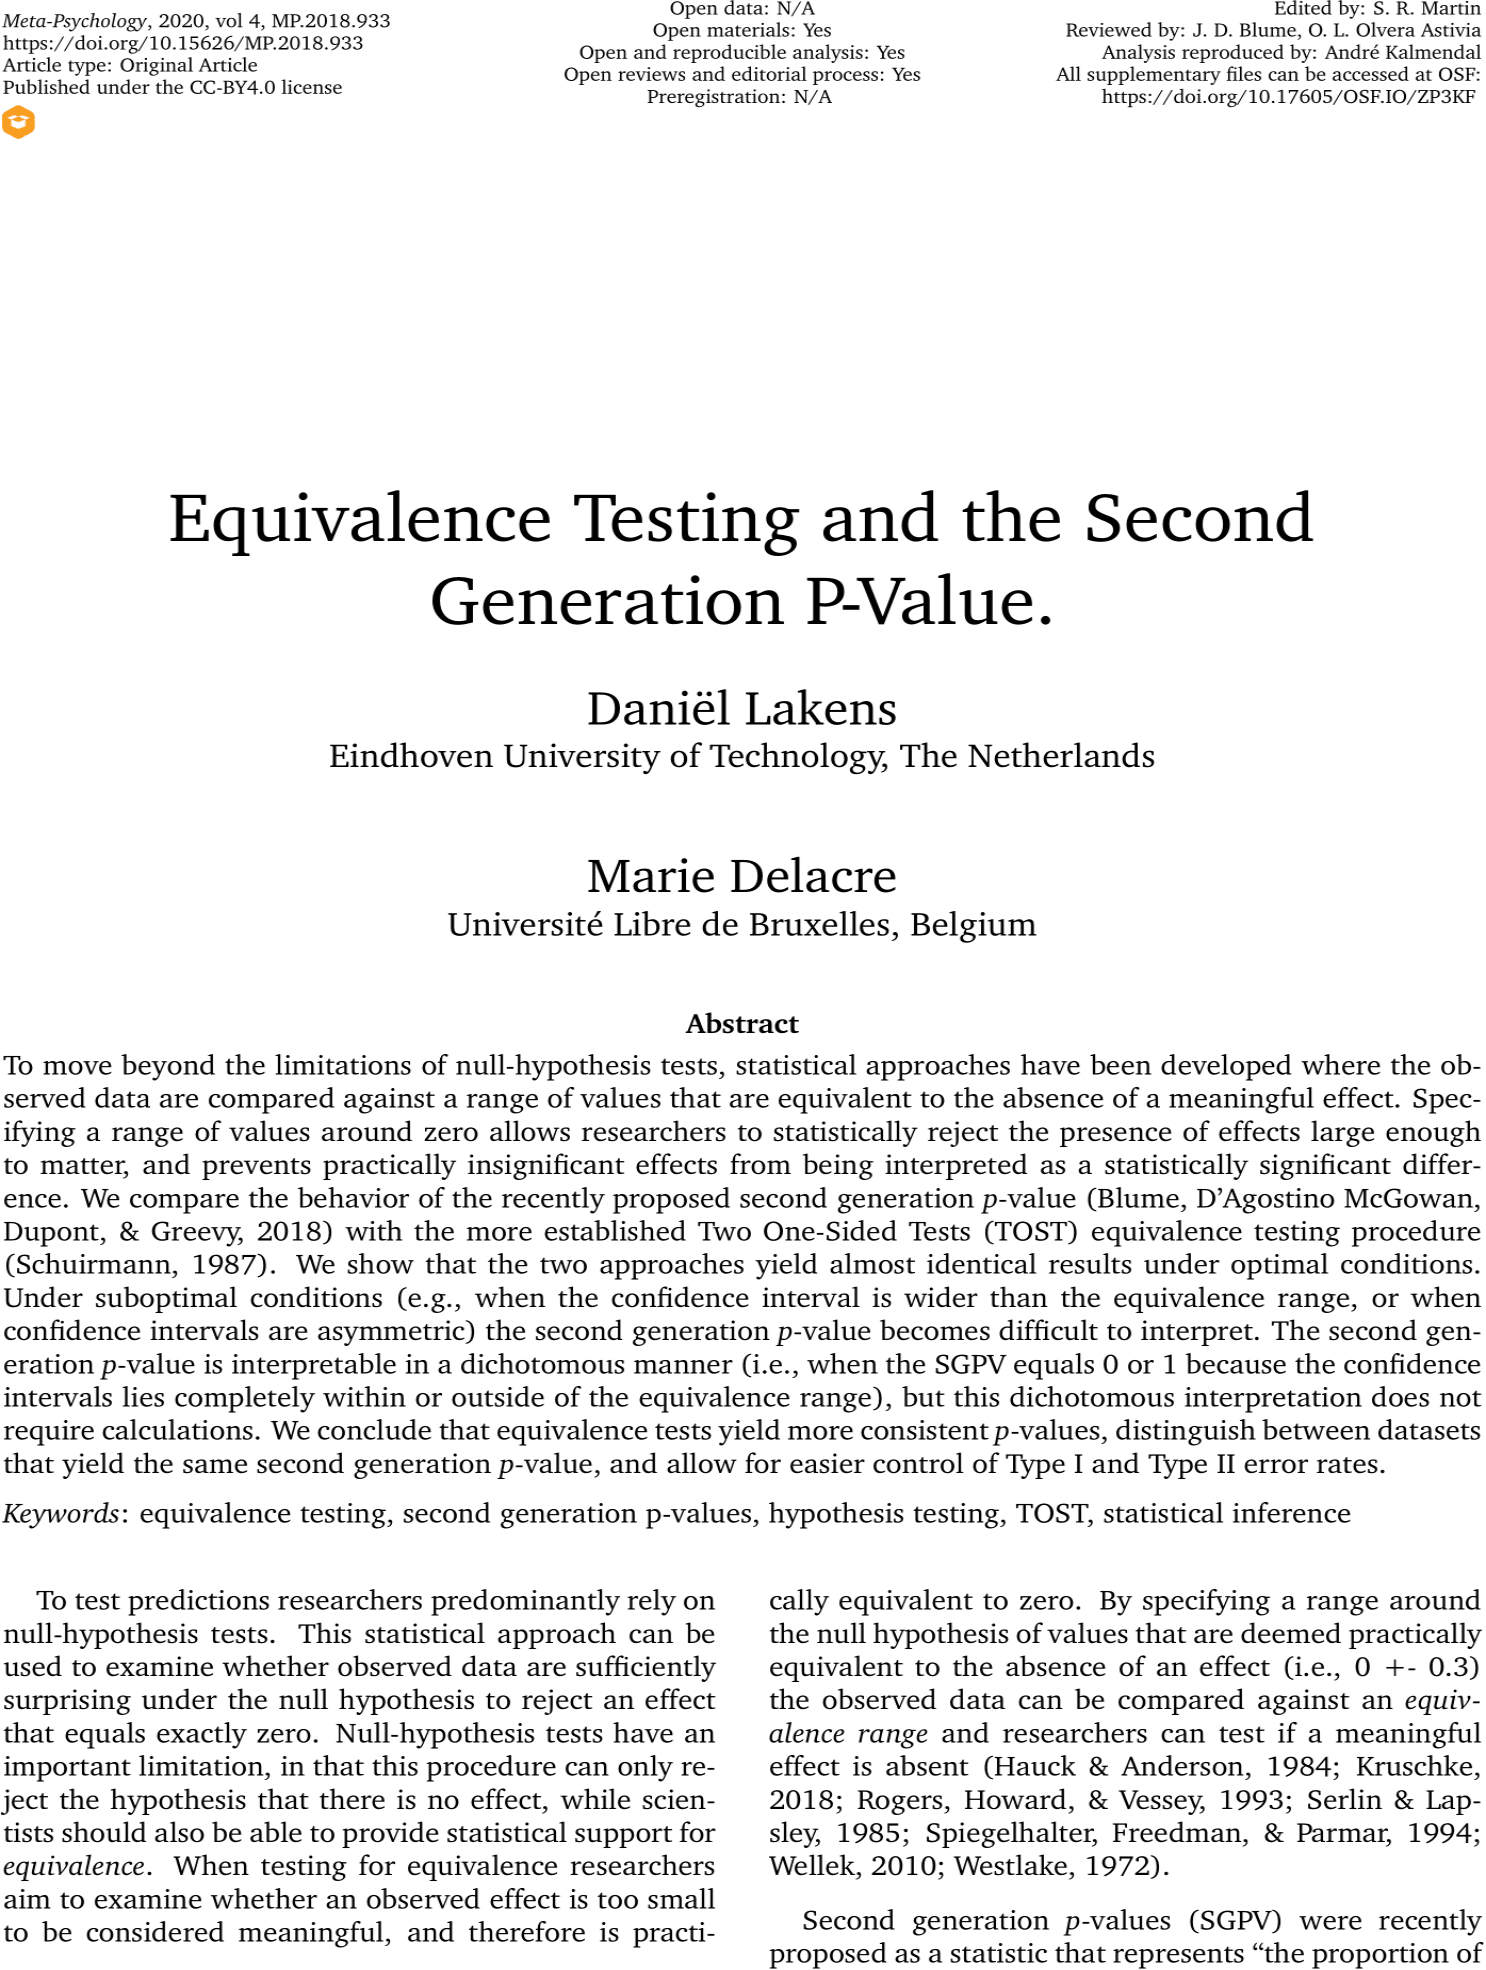
\includegraphics[width=0.92\linewidth]{C:/Users/Admin/OneDrive/Documents/Github projects/thesis/Chapitre 5/Chapitre 5-1} \end{center}

\begin{center}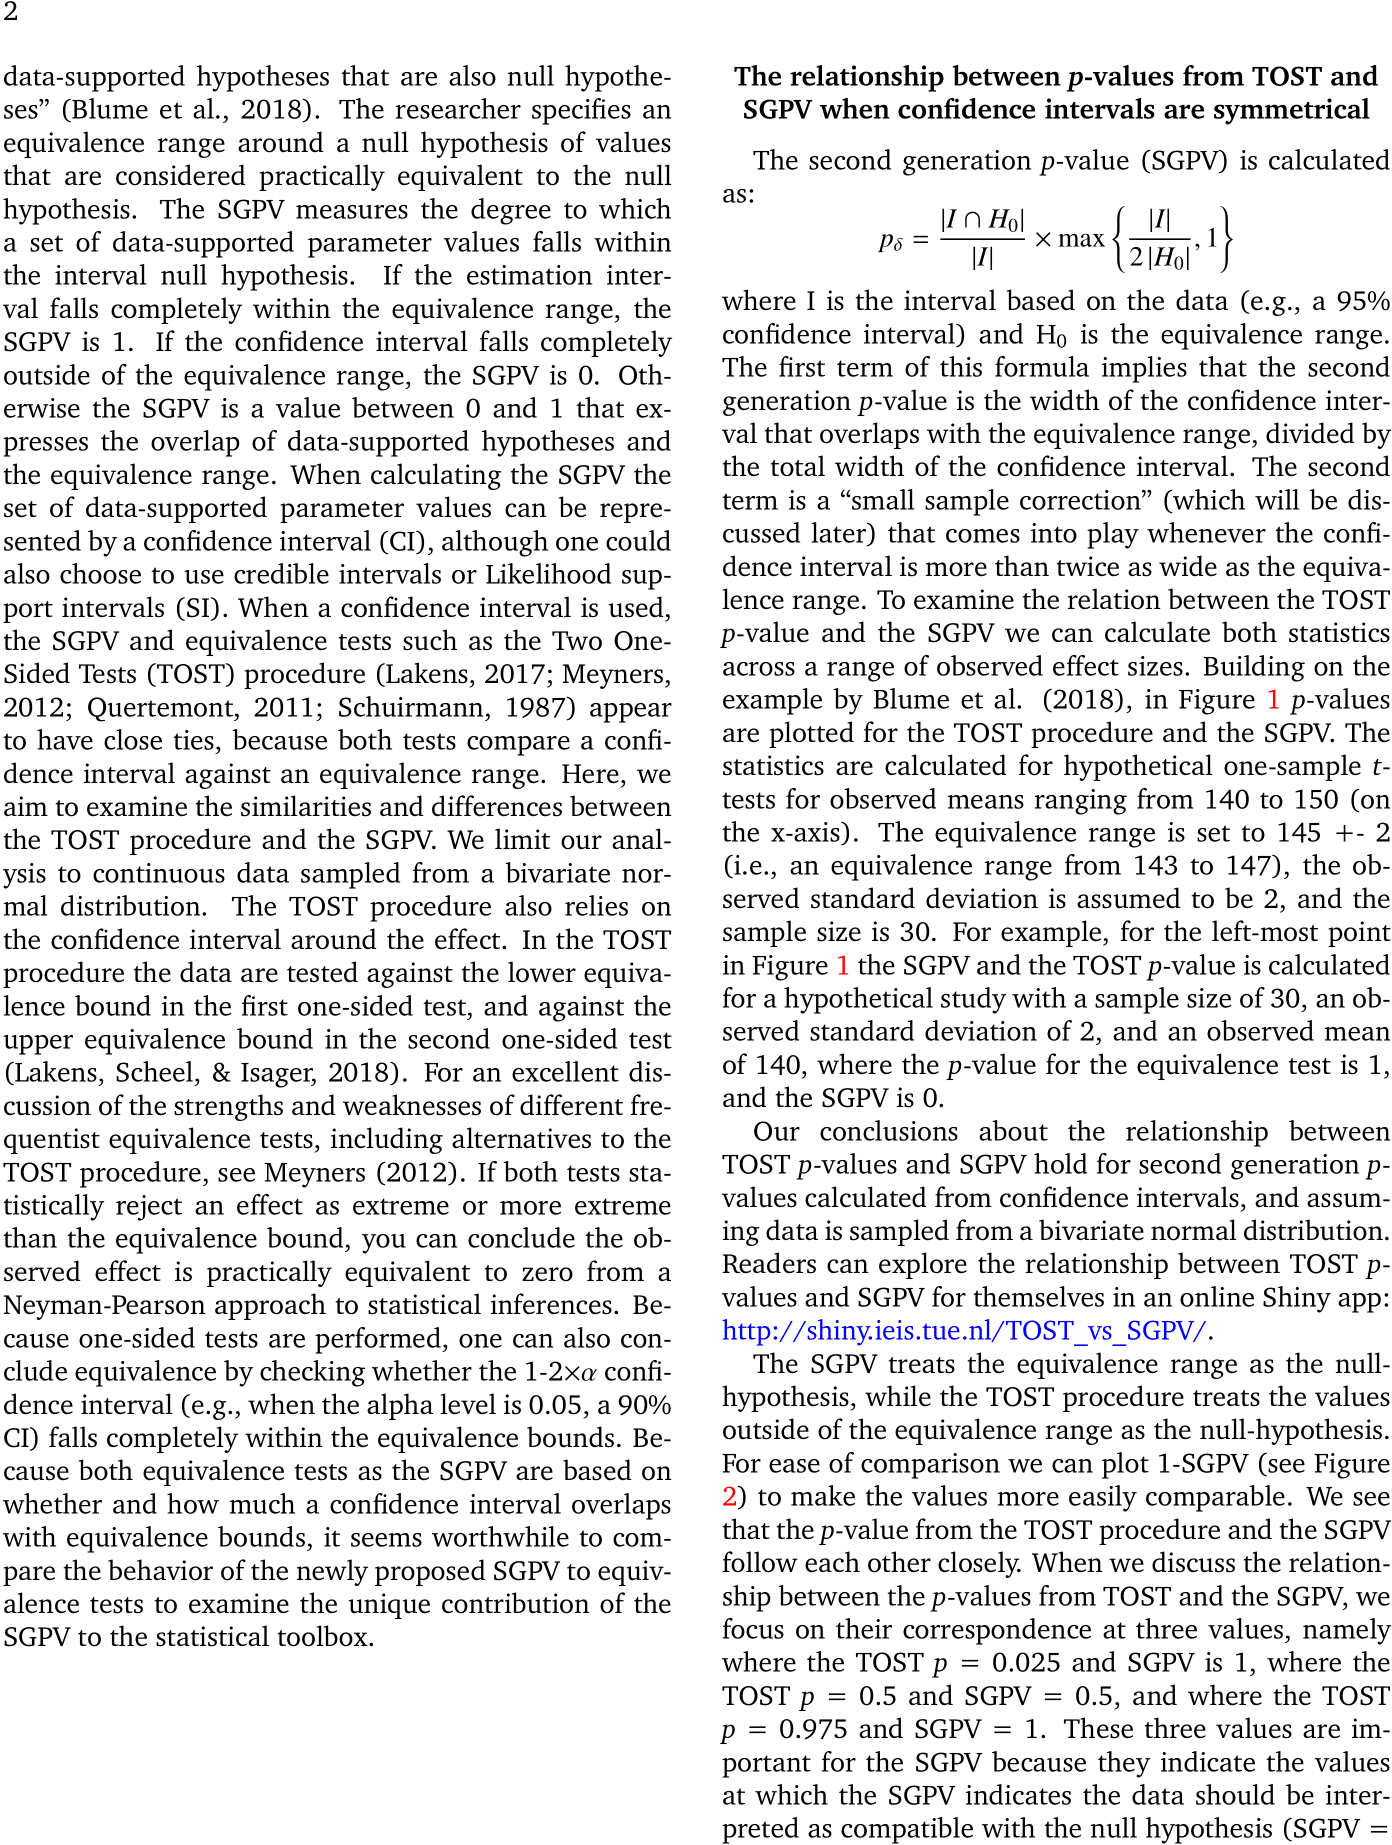
\includegraphics[width=5.51in]{C:/Users/Admin/OneDrive/Documents/Github projects/thesis/Chapitre 5/Chapitre 5-2} \end{center}

\begin{center}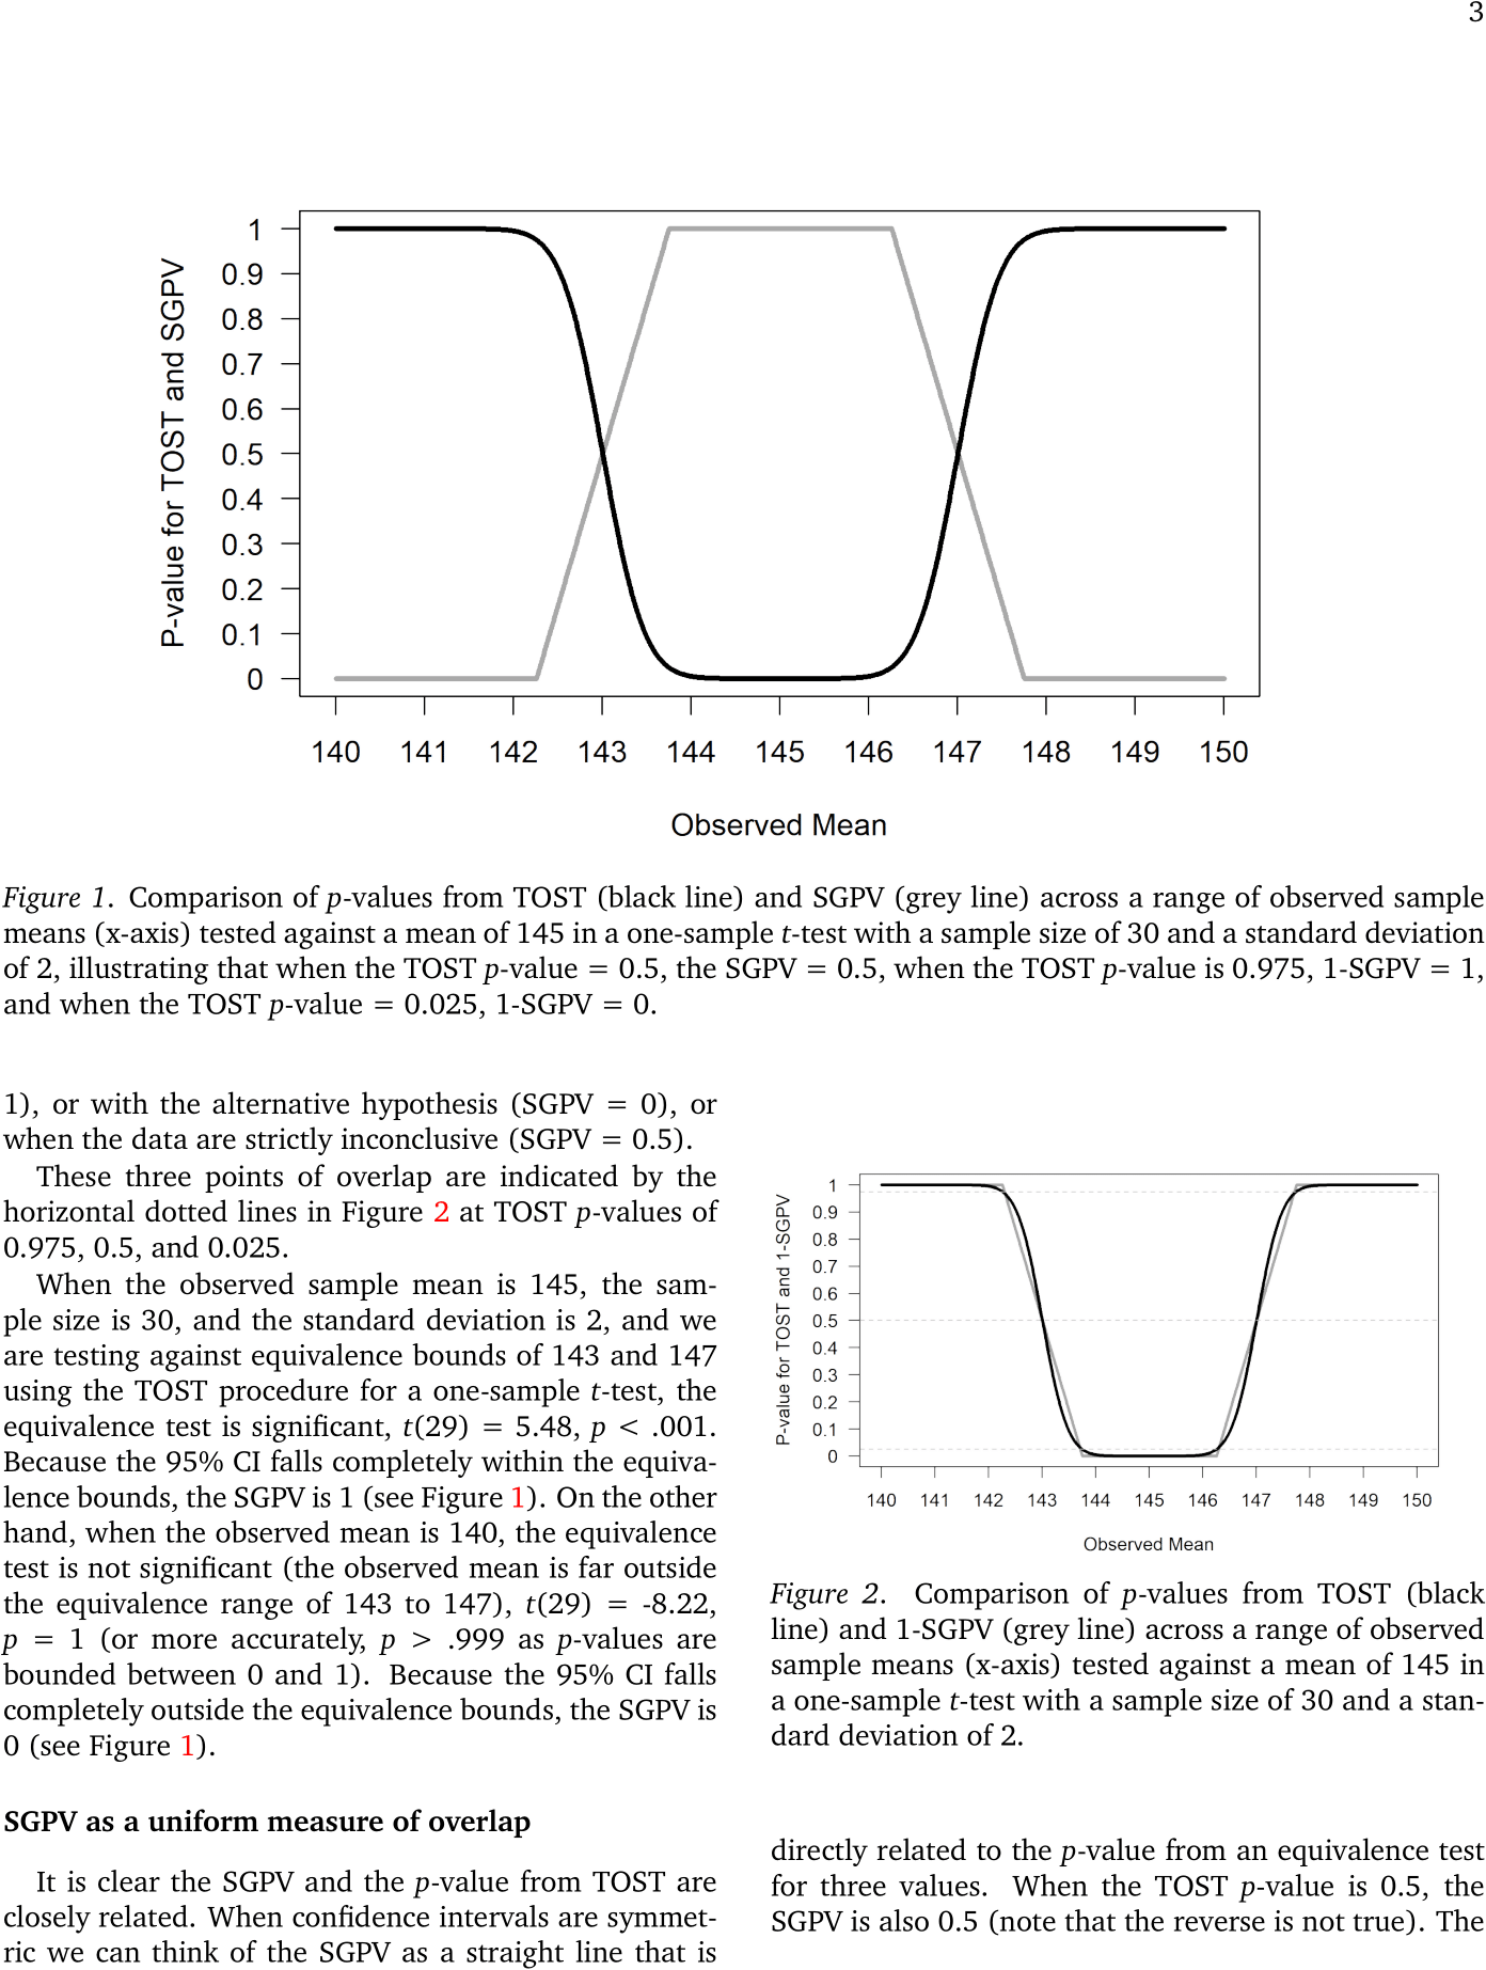
\includegraphics[width=5.51in]{C:/Users/Admin/OneDrive/Documents/Github projects/thesis/Chapitre 5/Chapitre 5-3} \end{center}

\begin{center}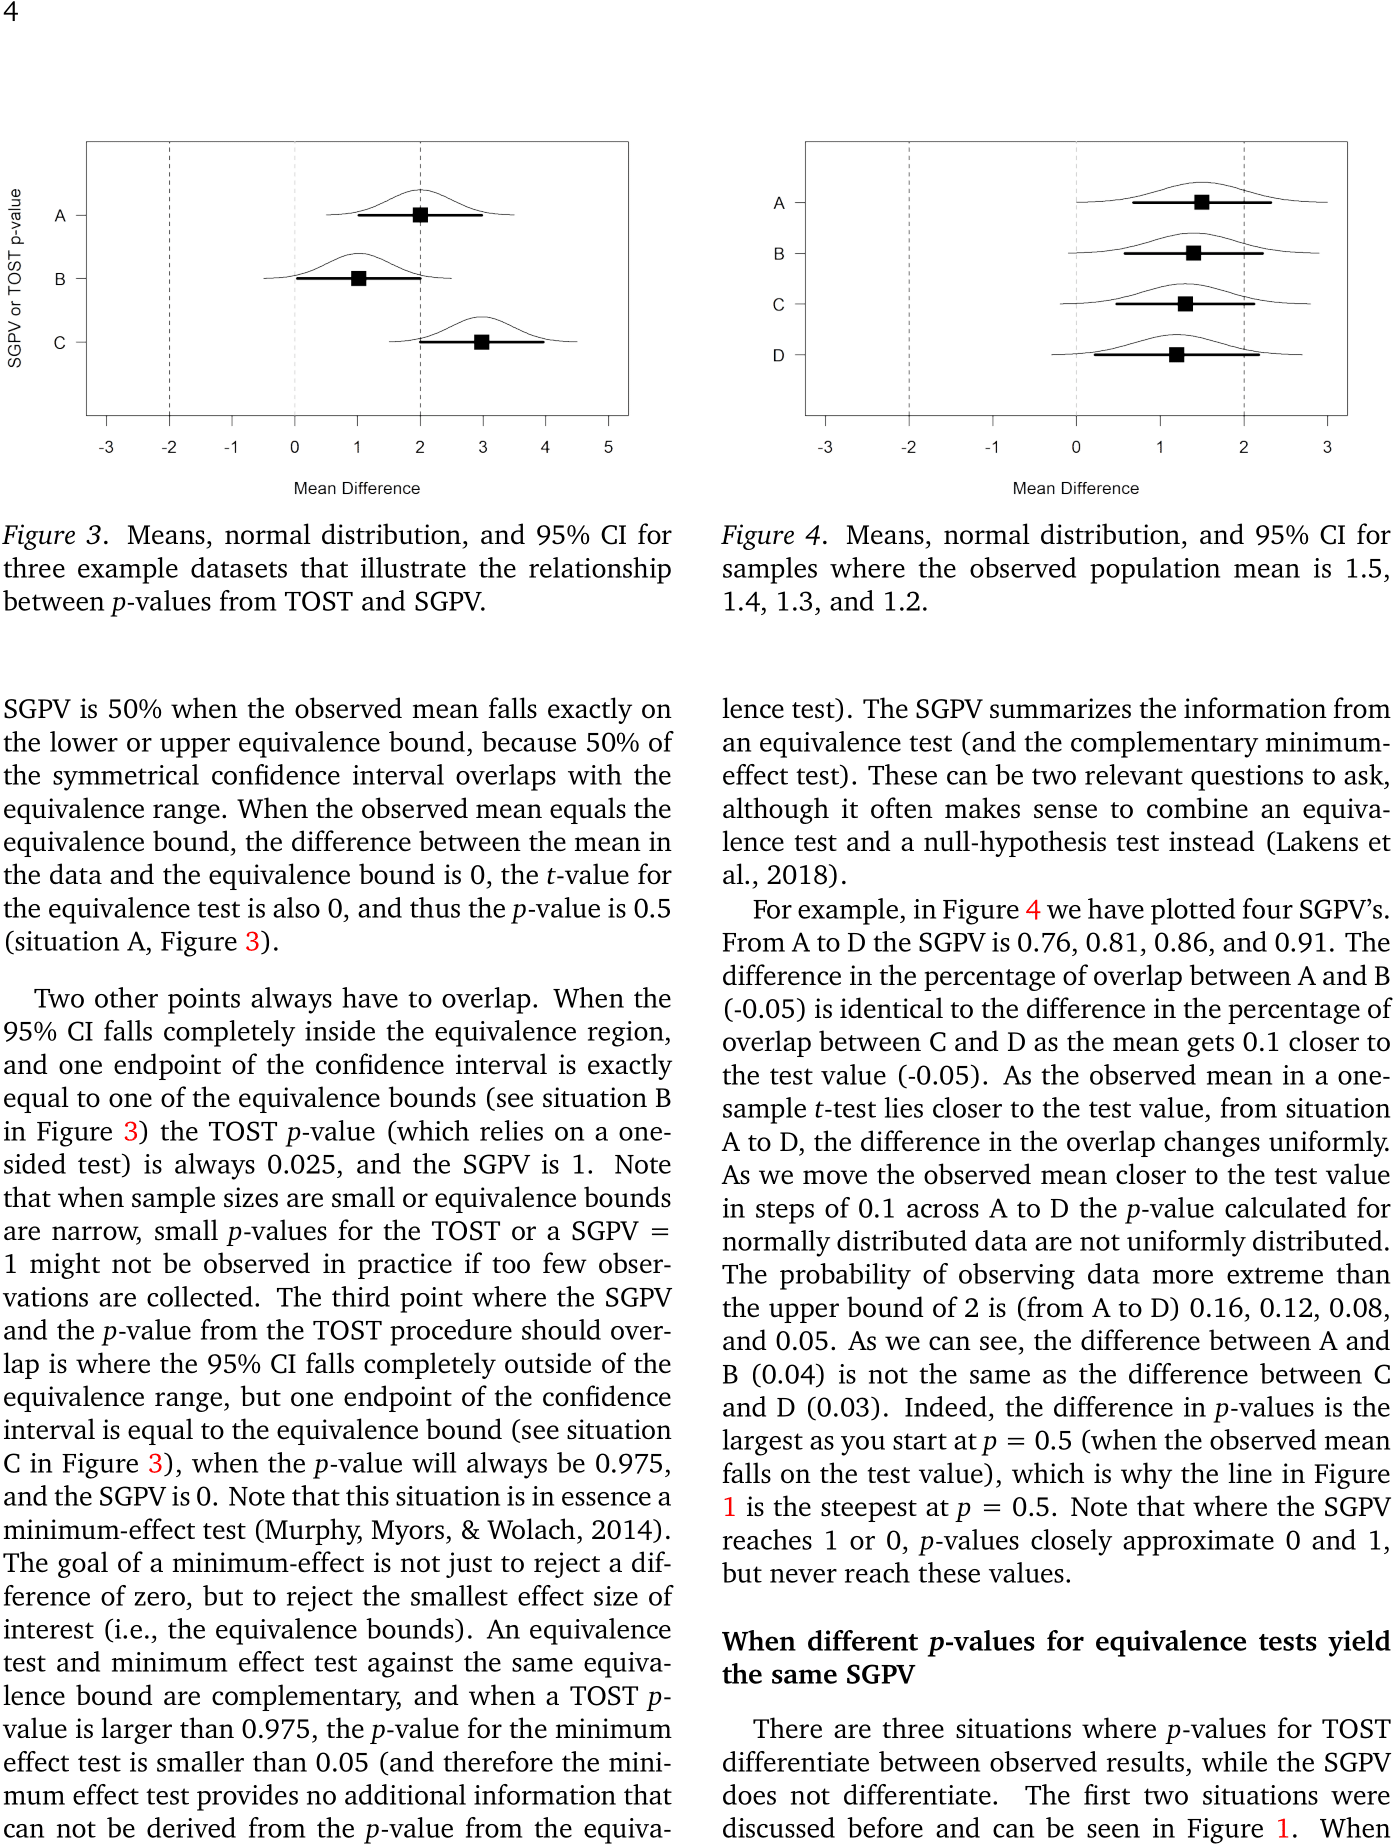
\includegraphics[width=5.51in]{C:/Users/Admin/OneDrive/Documents/Github projects/thesis/Chapitre 5/Chapitre 5-4} \end{center}

\begin{center}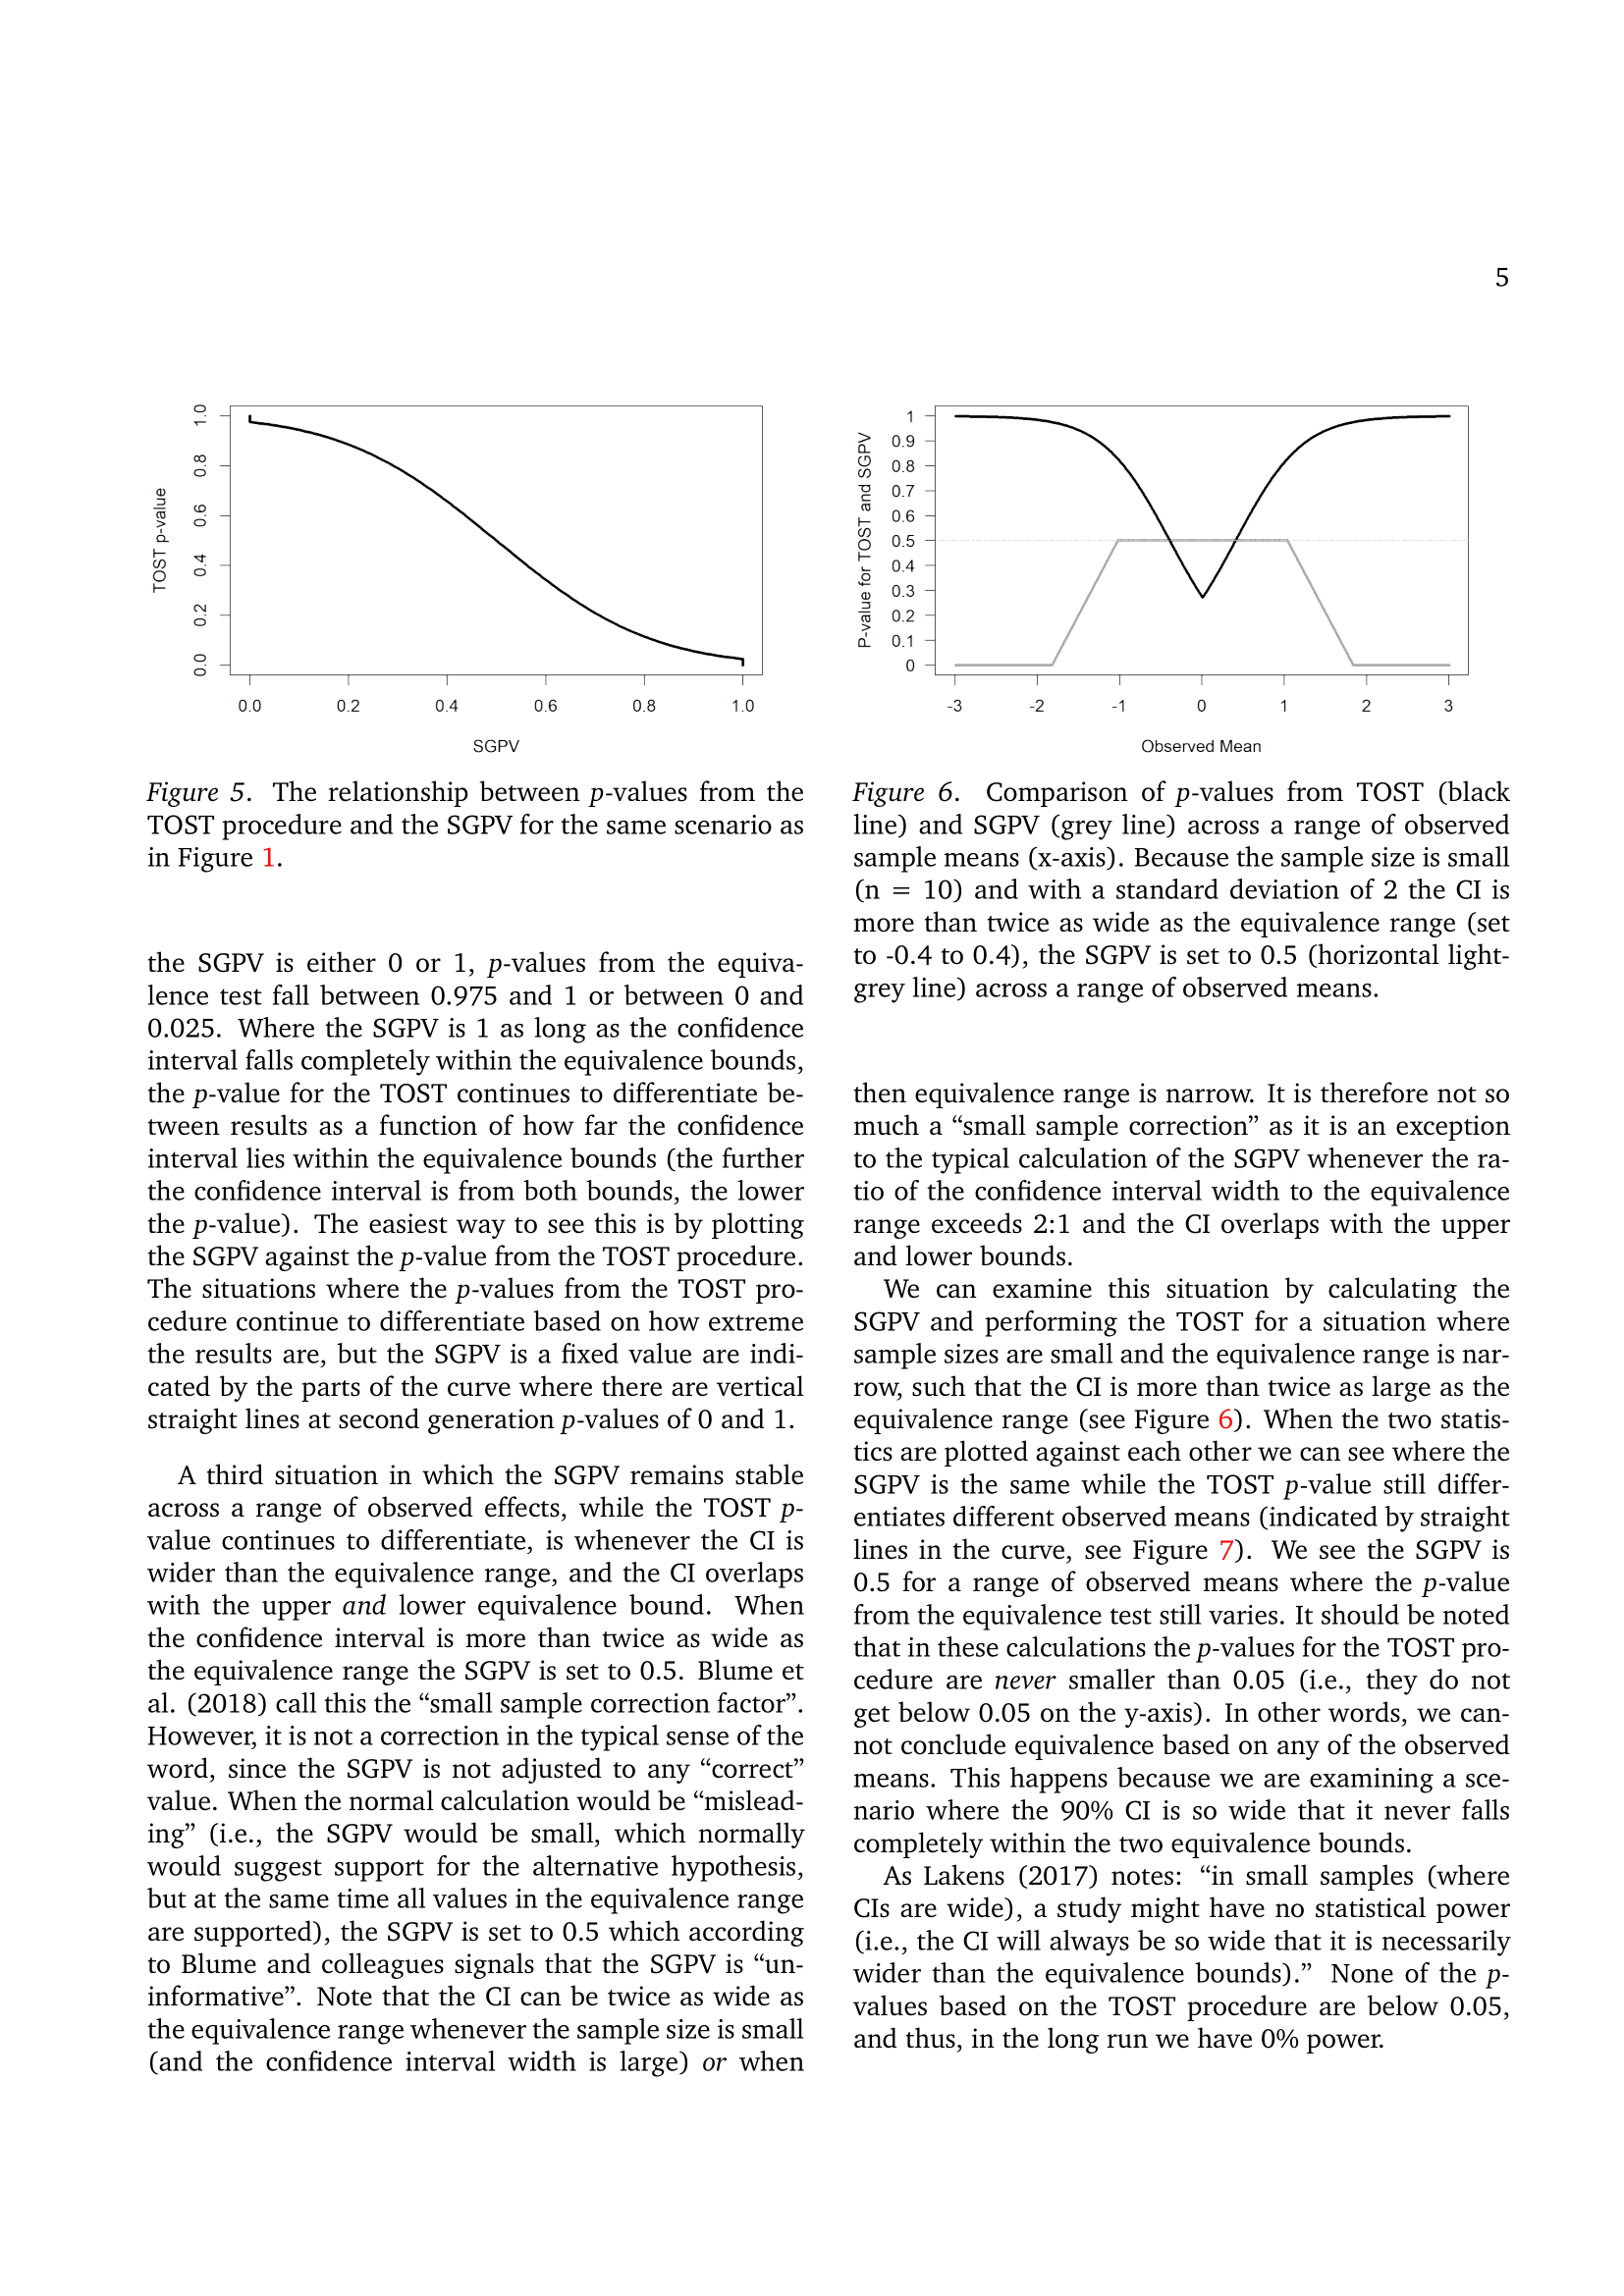
\includegraphics[width=5.51in]{C:/Users/Admin/OneDrive/Documents/Github projects/thesis/Chapitre 5/Chapitre 5-5} \end{center}

\begin{center}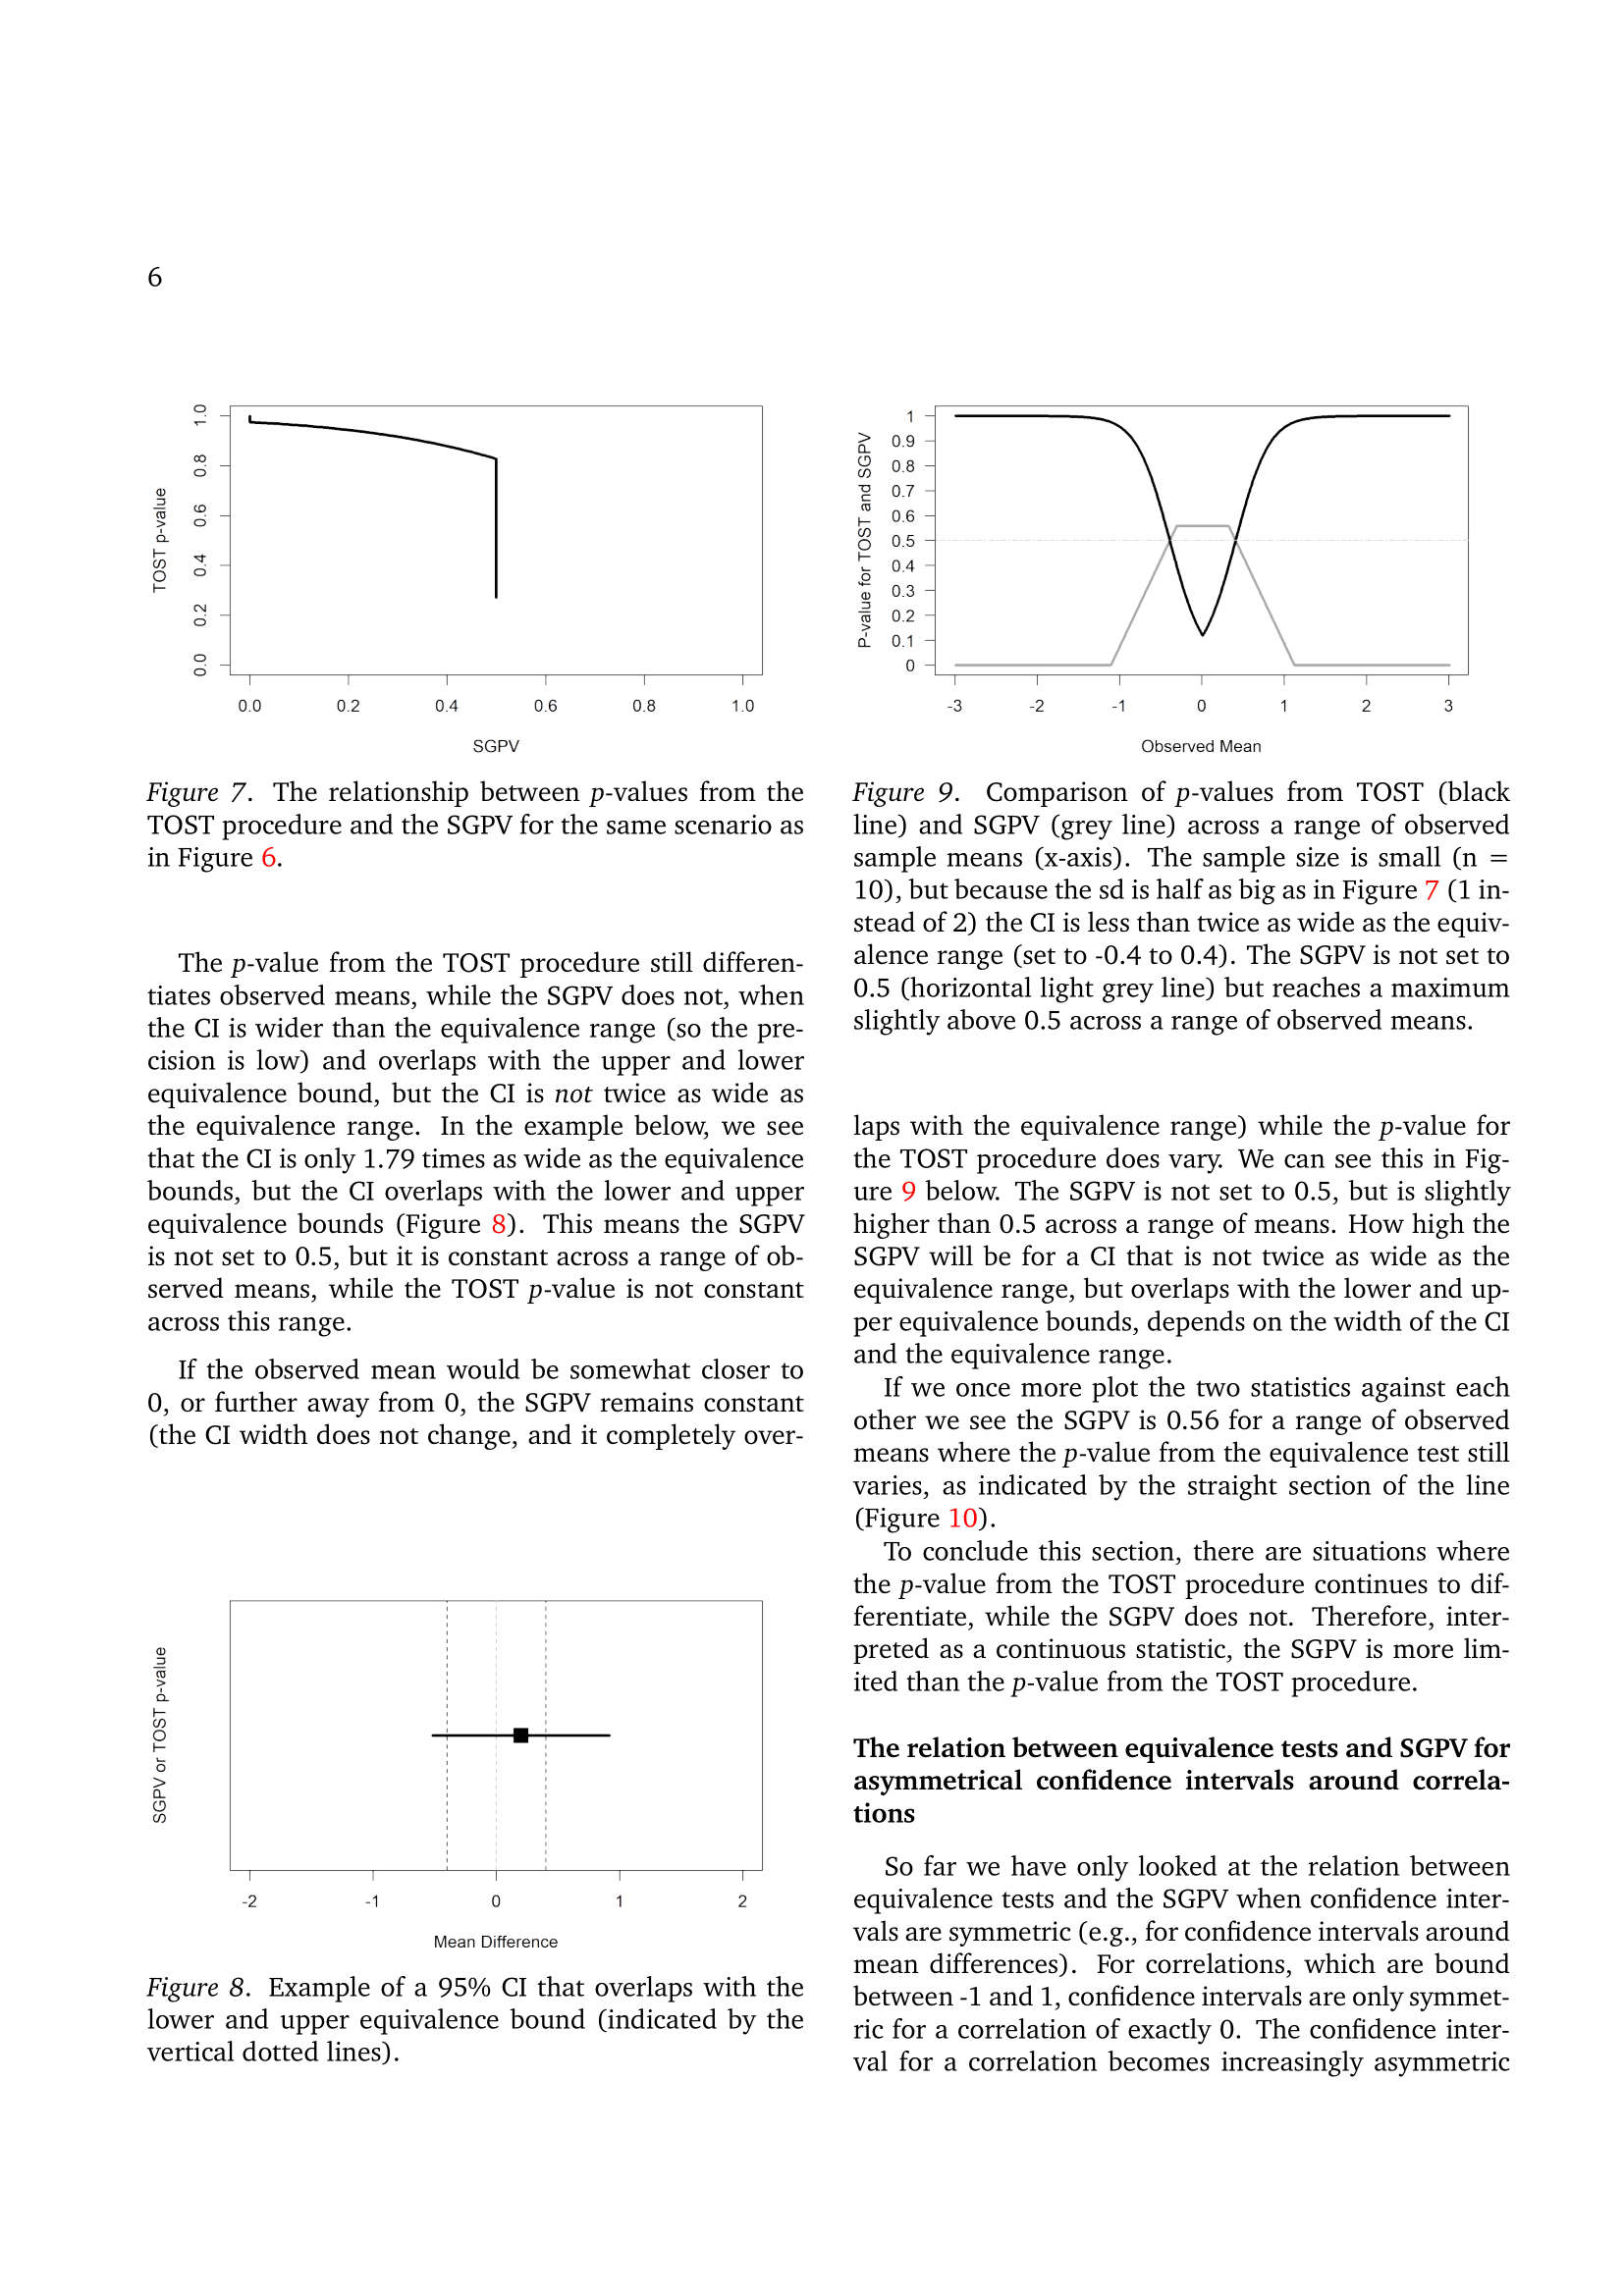
\includegraphics[width=5.51in]{C:/Users/Admin/OneDrive/Documents/Github projects/thesis/Chapitre 5/Chapitre 5-6} \end{center}

\begin{center}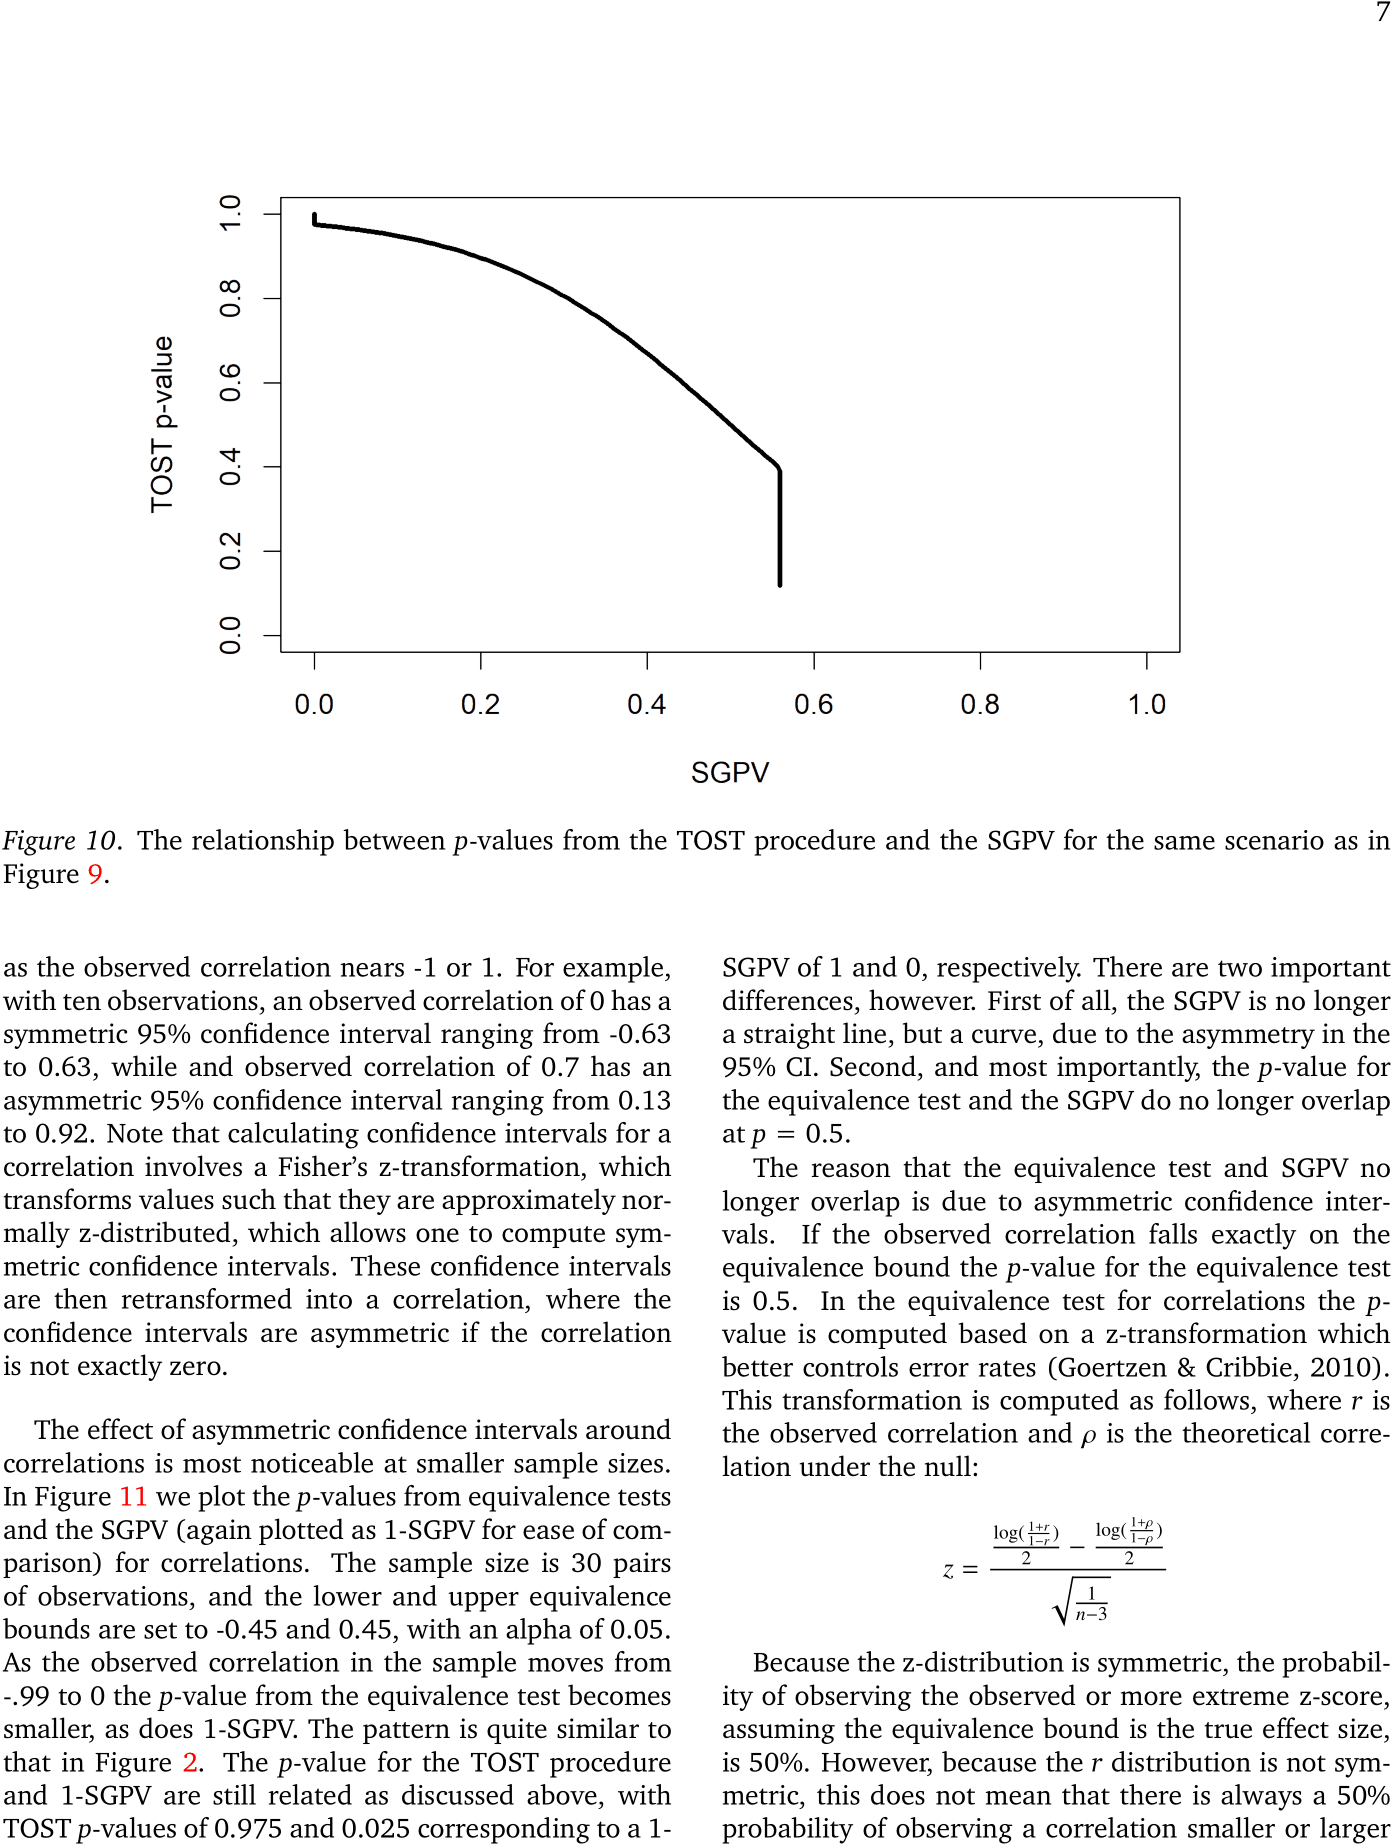
\includegraphics[width=5.51in]{C:/Users/Admin/OneDrive/Documents/Github projects/thesis/Chapitre 5/Chapitre 5-7} \end{center}

\begin{center}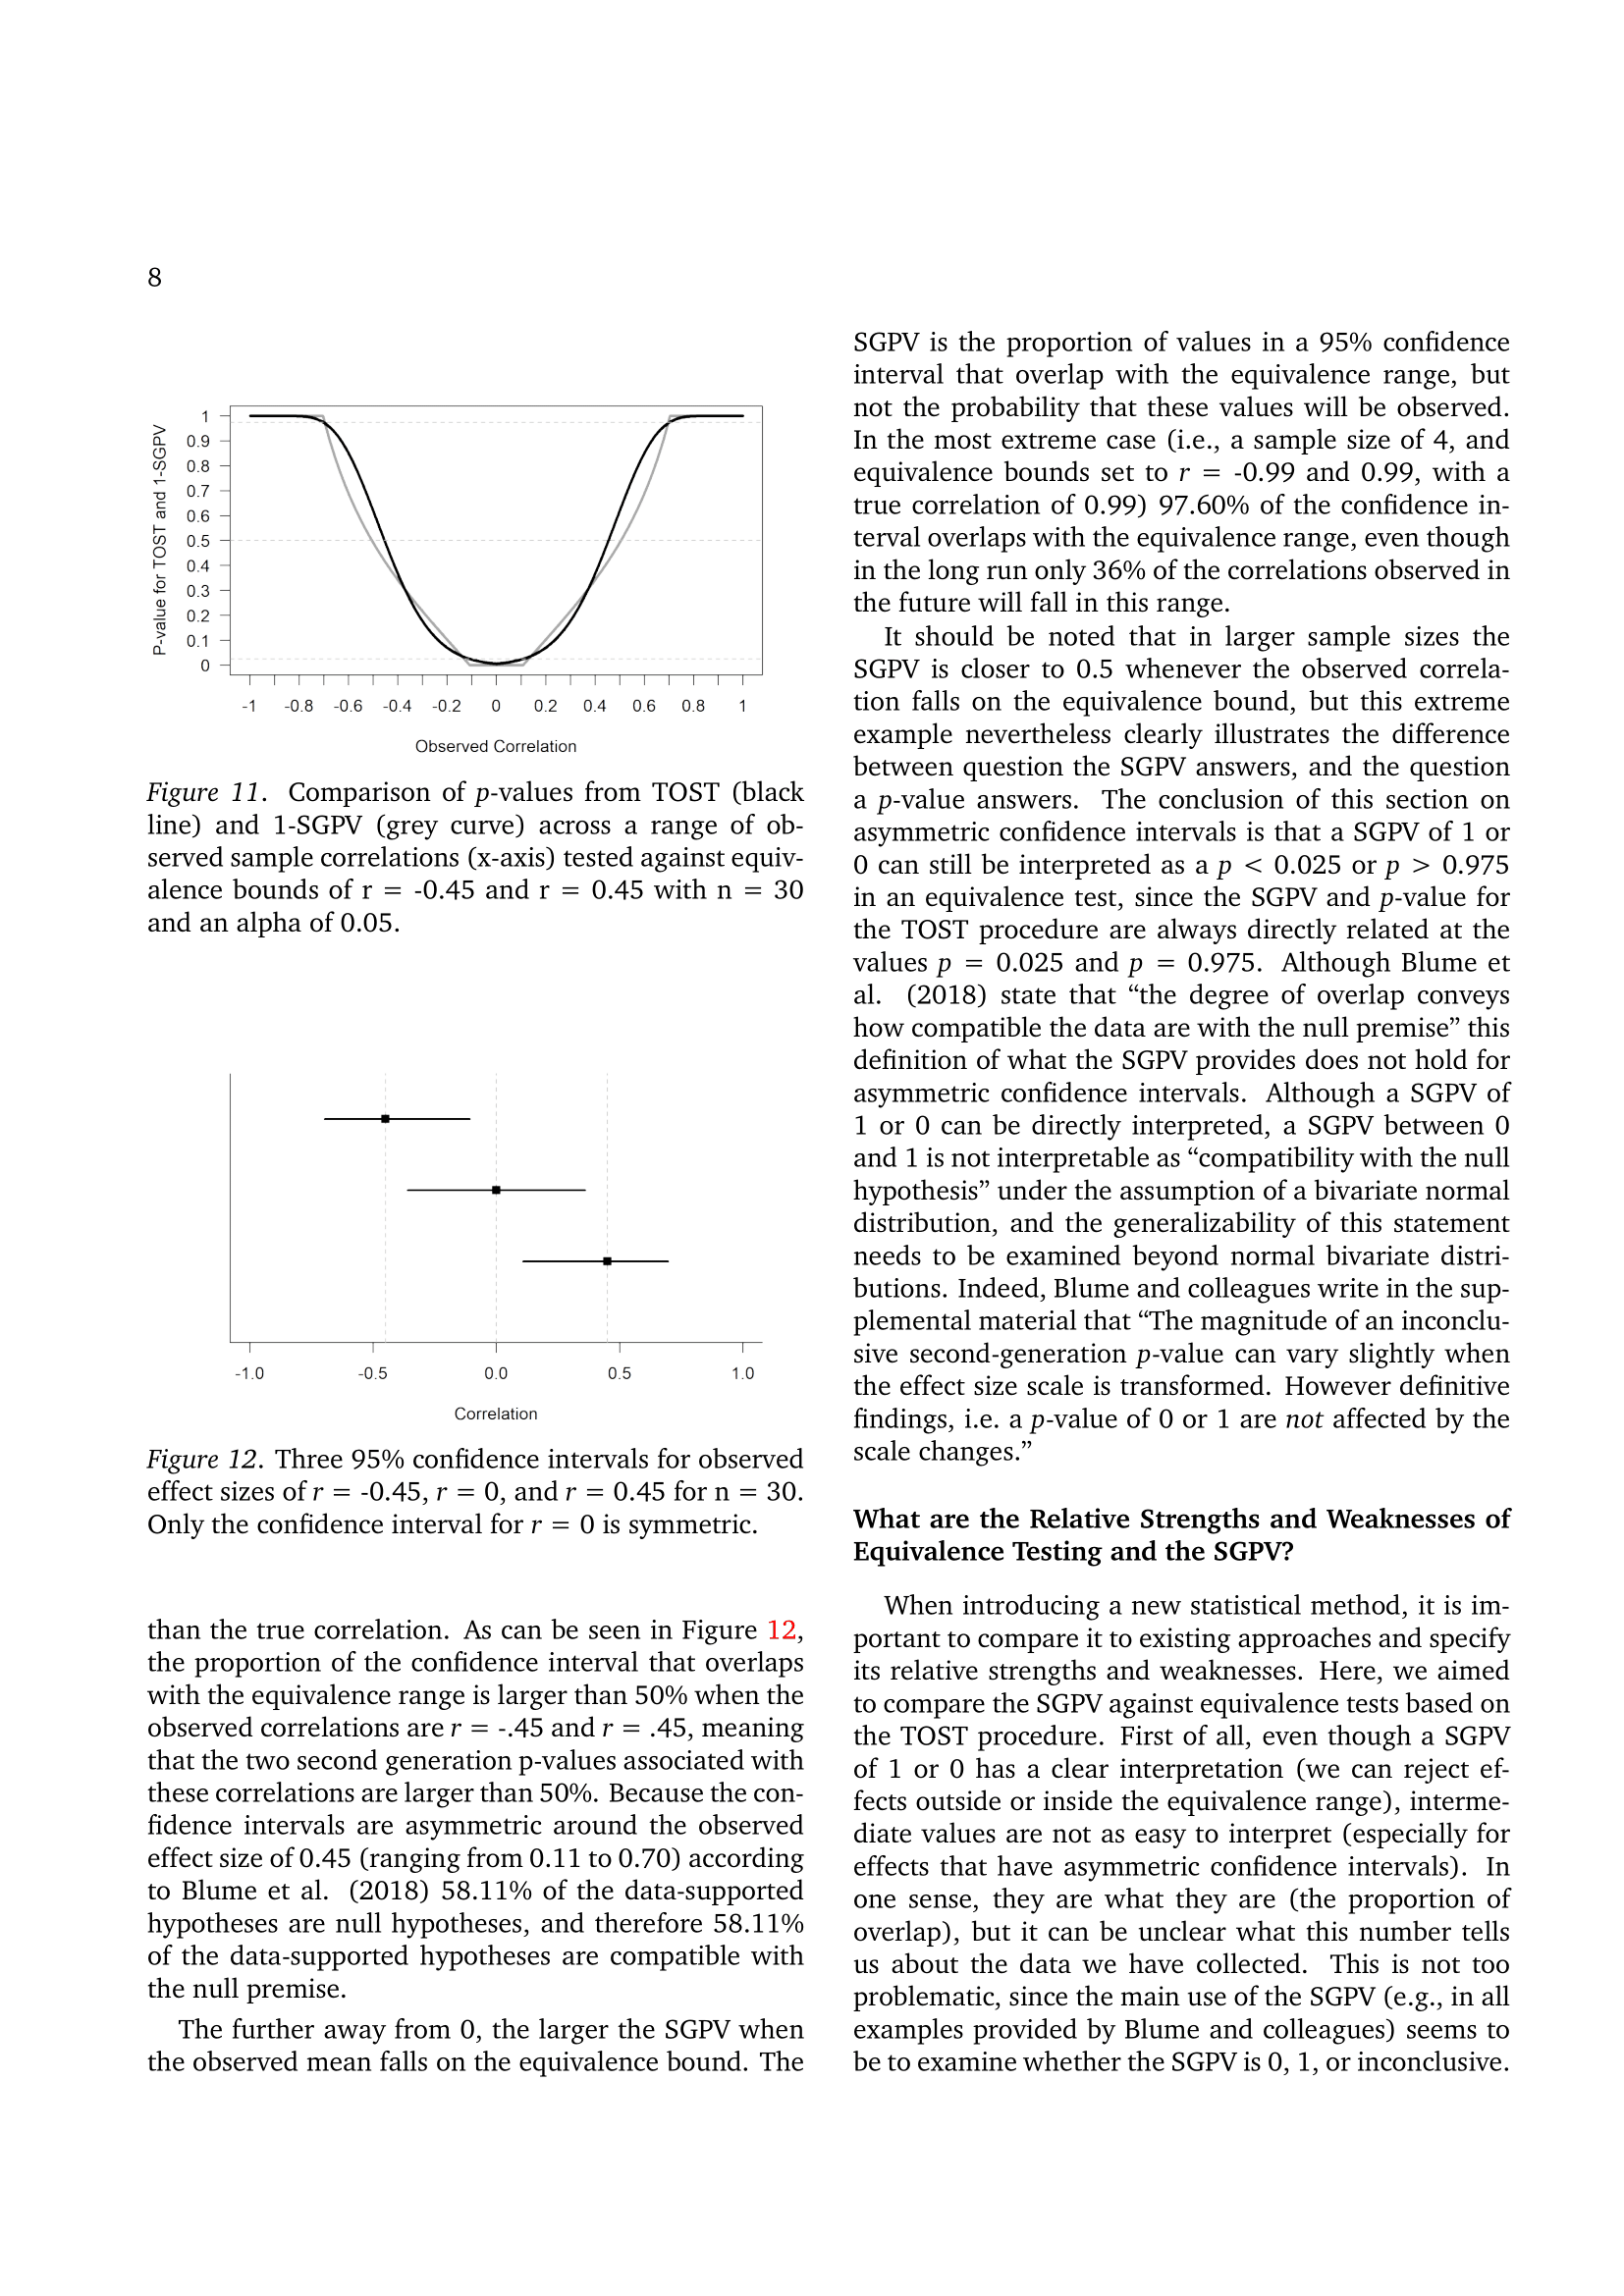
\includegraphics[width=5.51in]{C:/Users/Admin/OneDrive/Documents/Github projects/thesis/Chapitre 5/Chapitre 5-8} \end{center}

\begin{center}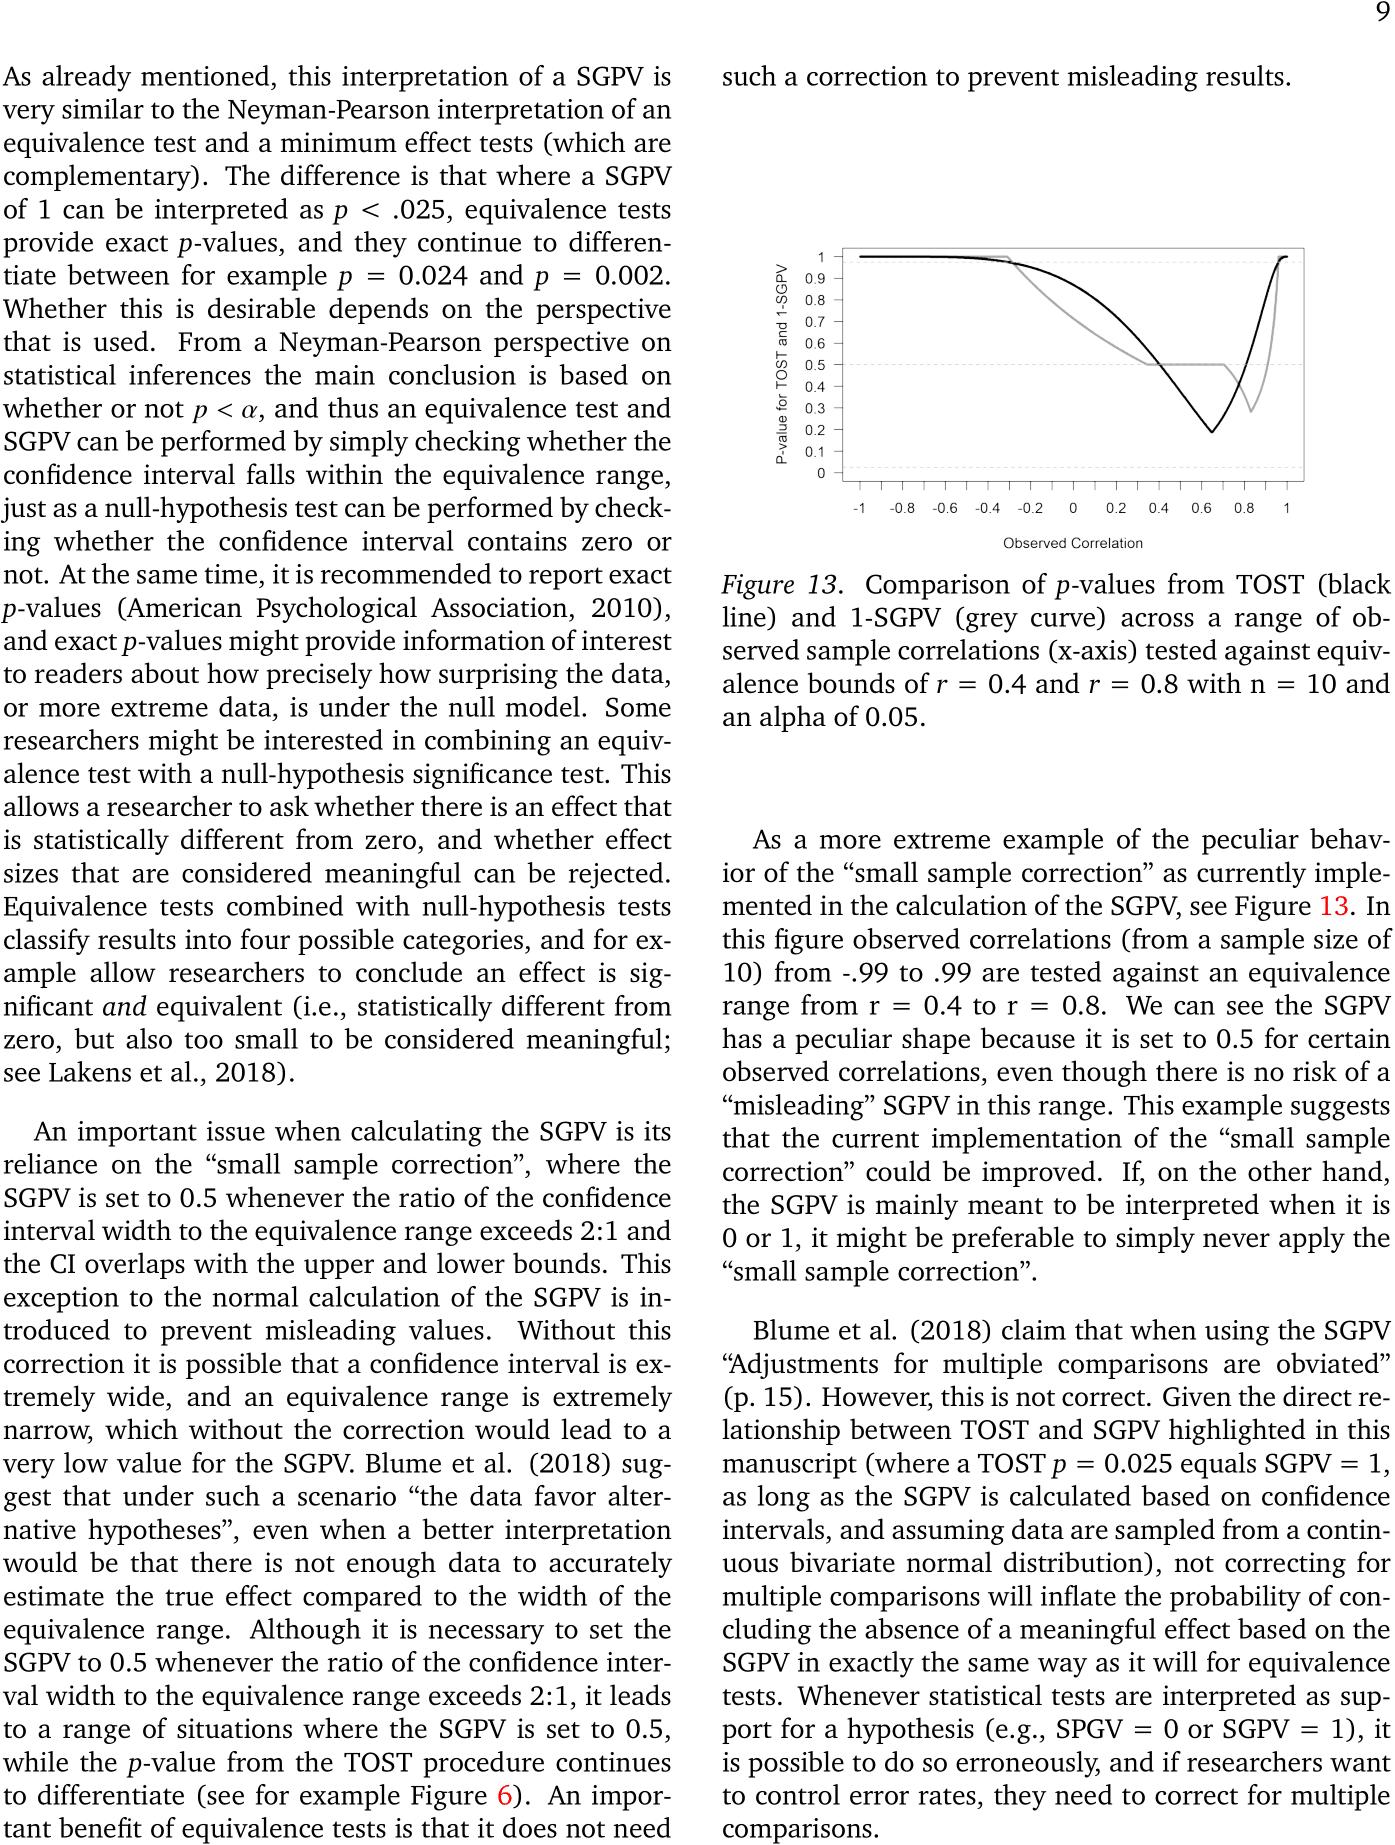
\includegraphics[width=5.51in]{C:/Users/Admin/OneDrive/Documents/Github projects/thesis/Chapitre 5/Chapitre 5-9} \end{center}

\begin{center}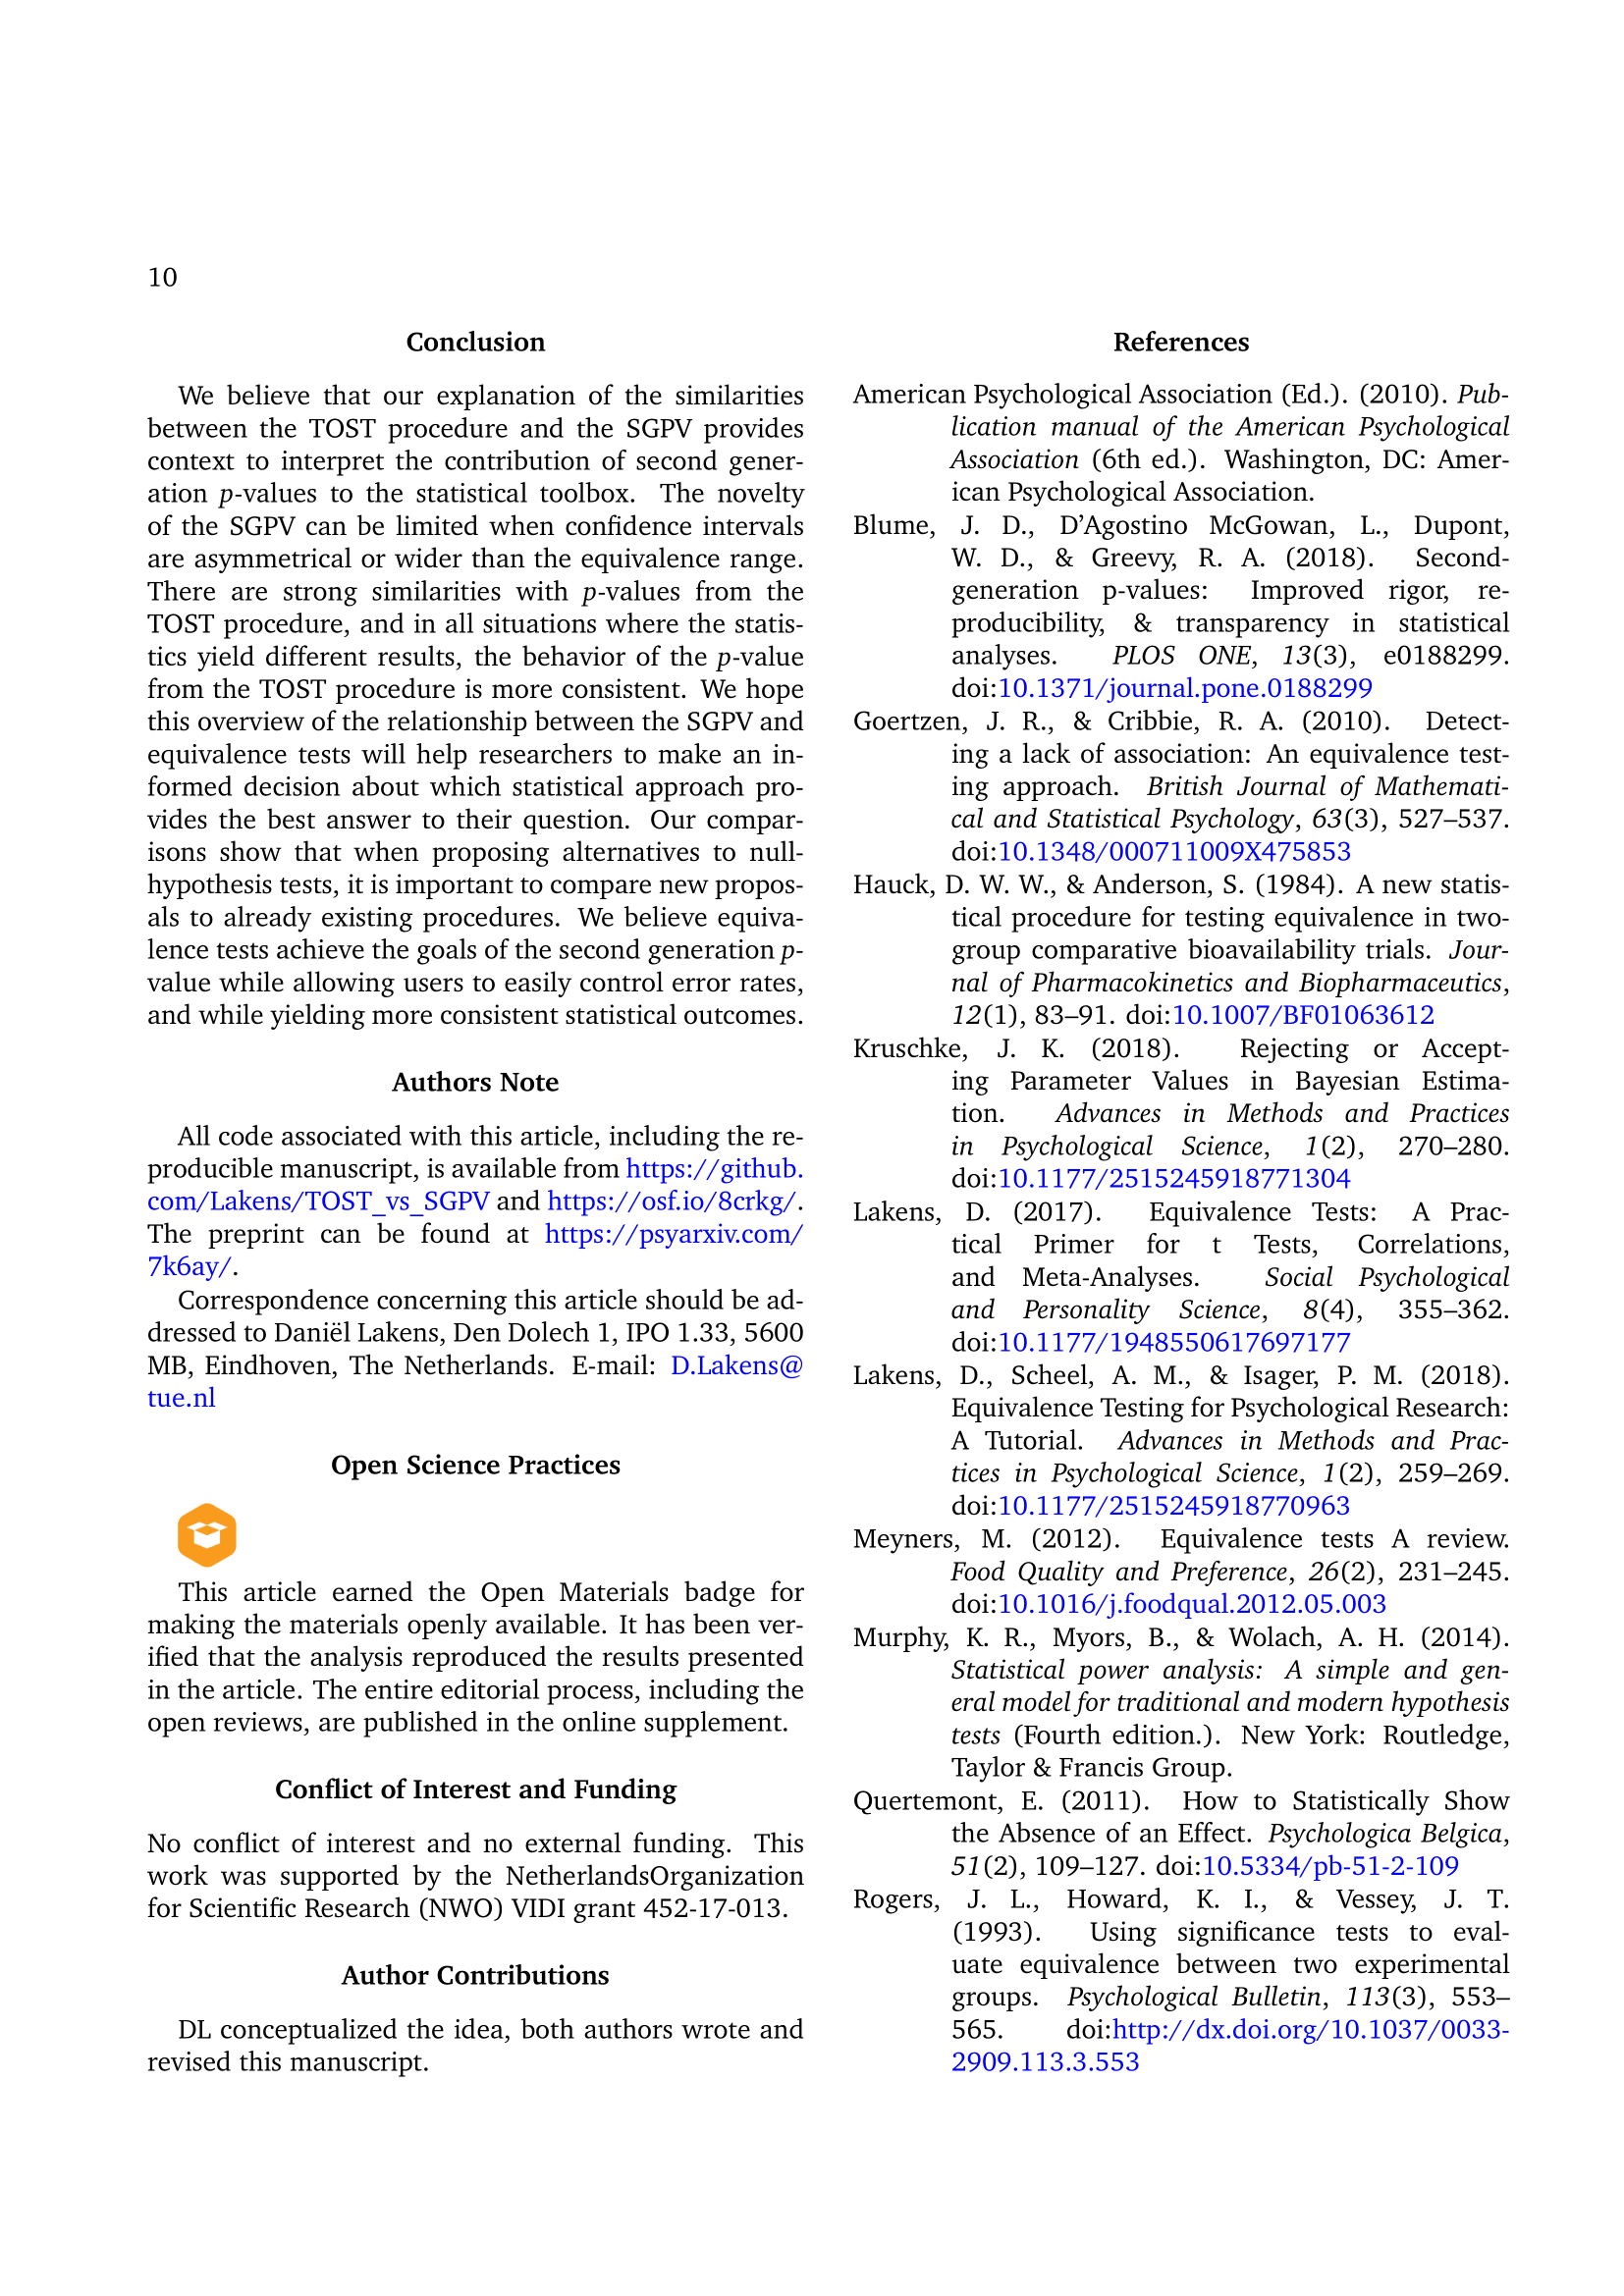
\includegraphics[width=5.51in]{C:/Users/Admin/OneDrive/Documents/Github projects/thesis/Chapitre 5/Chapitre 5-10} \end{center}

\begin{center}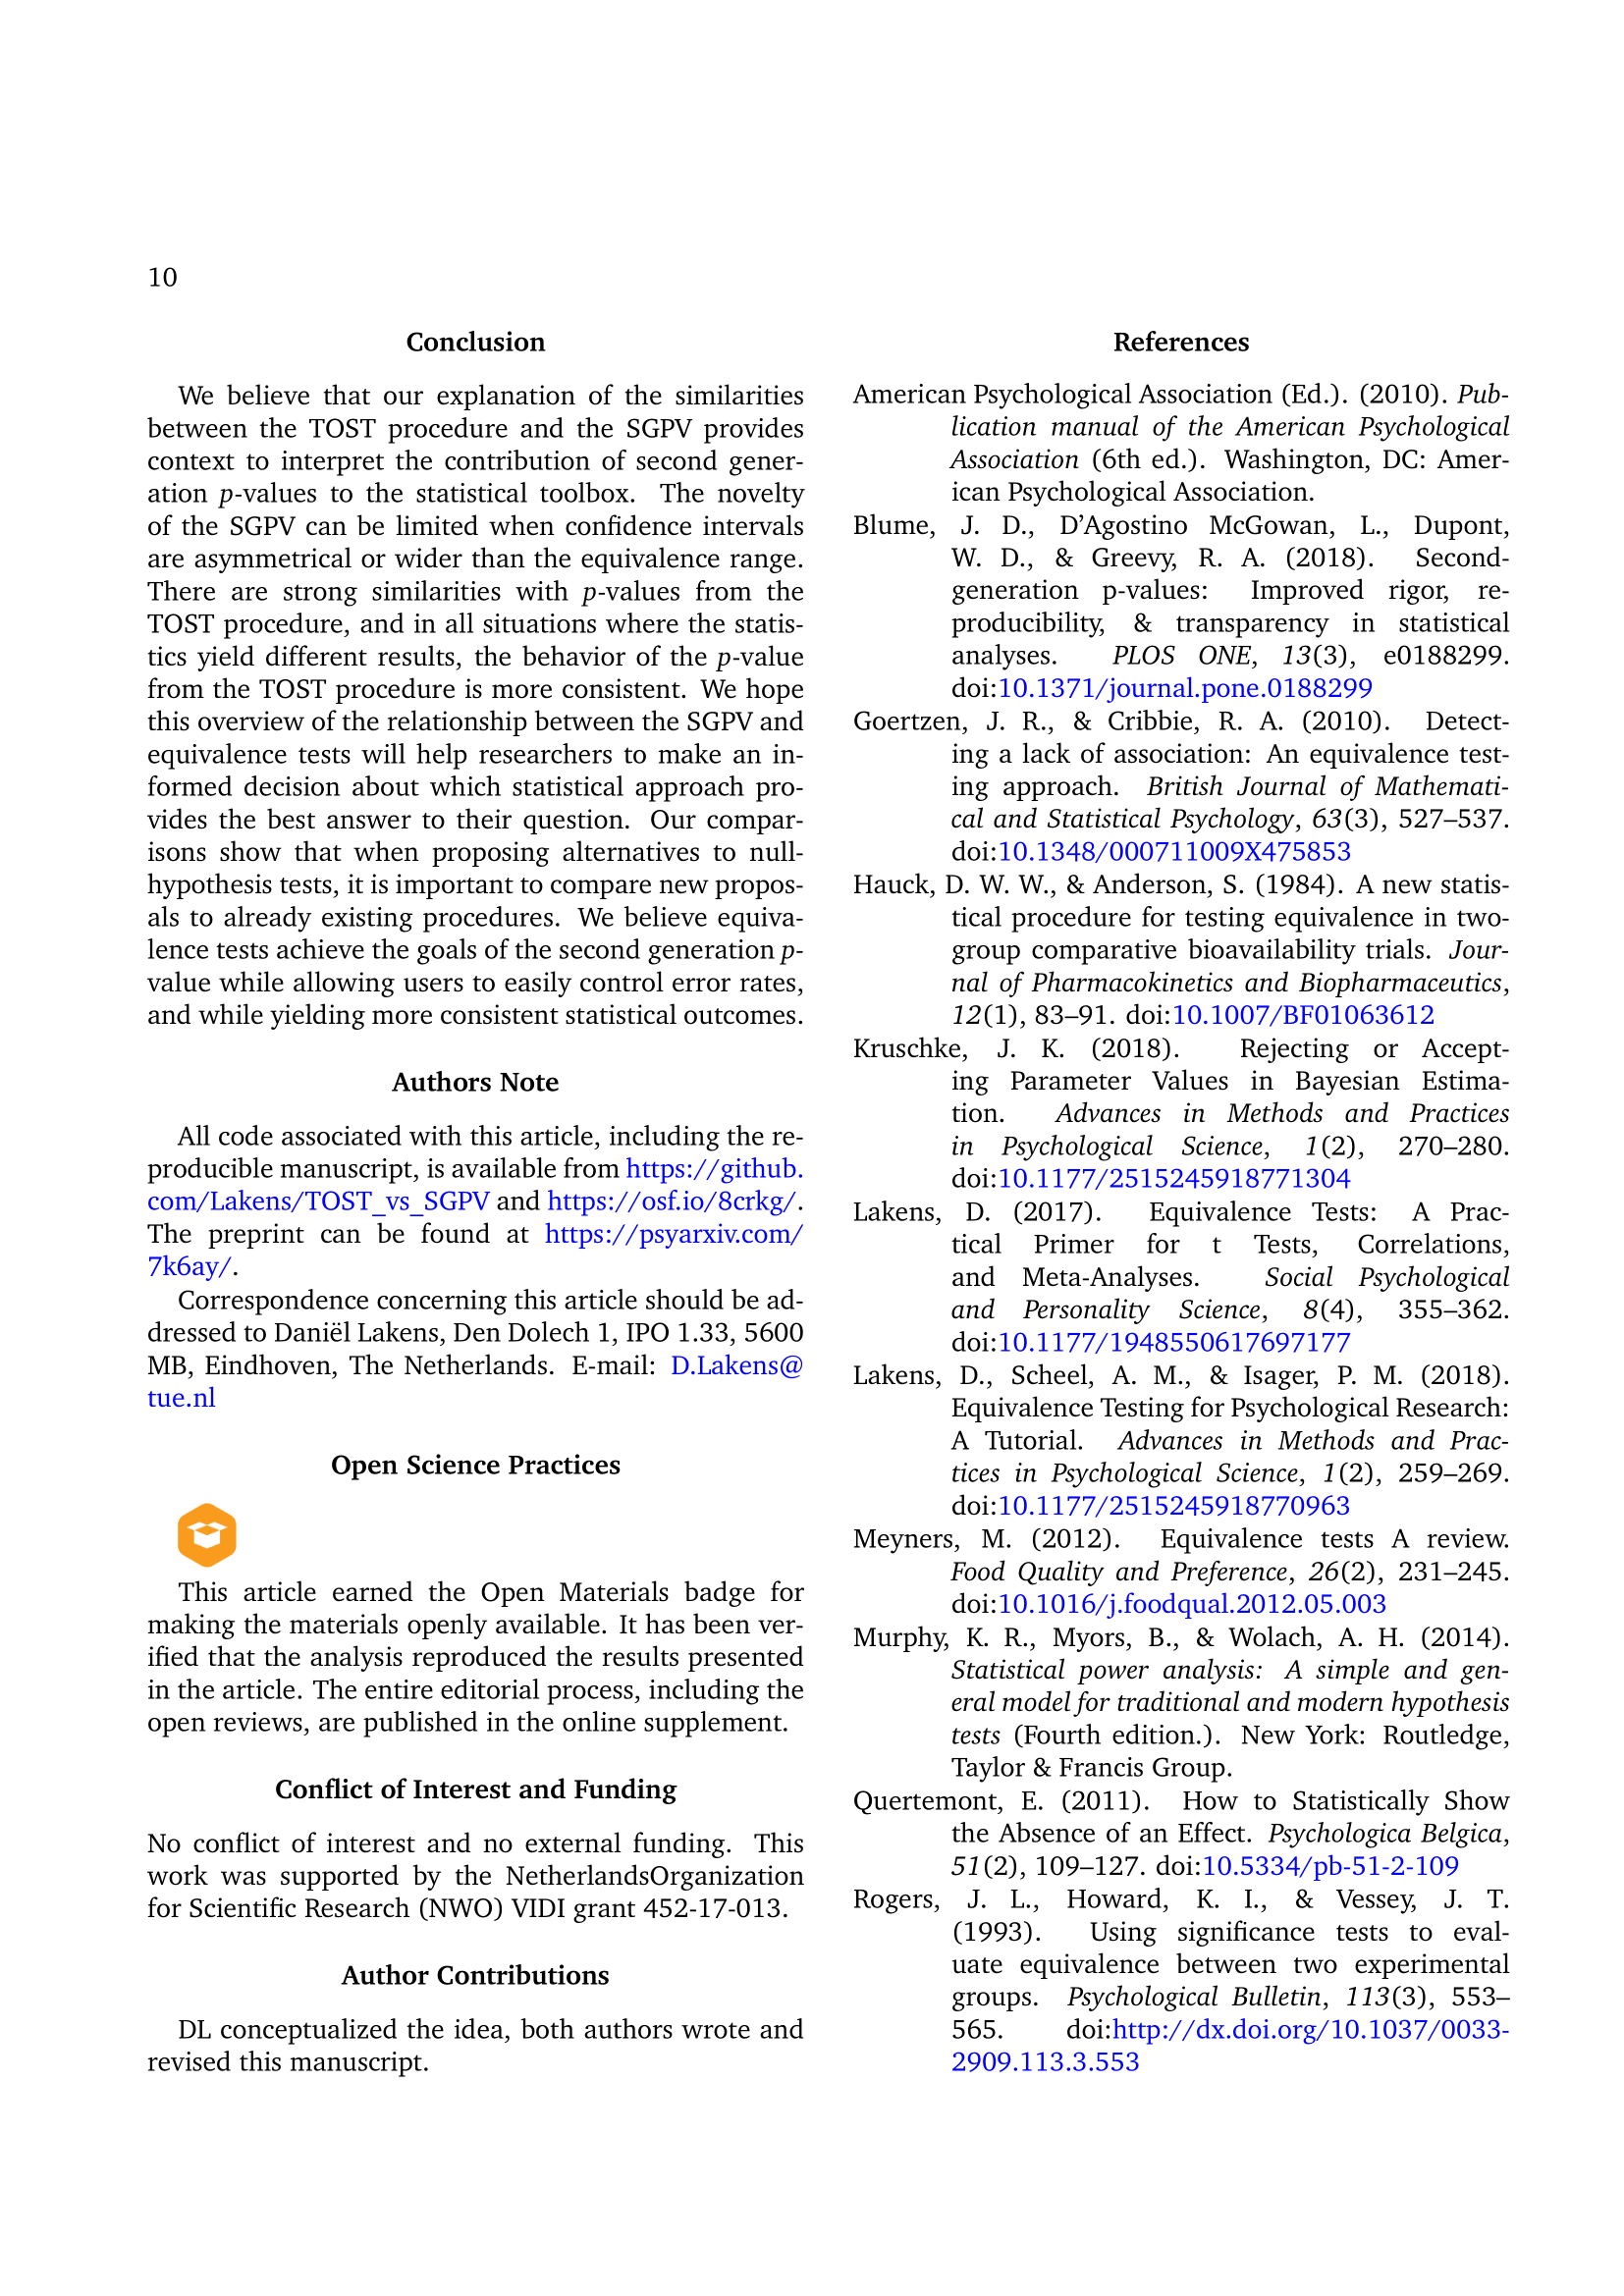
\includegraphics[width=5.51in]{C:/Users/Admin/OneDrive/Documents/Github projects/thesis/Chapitre 5/Chapitre 5-10} \end{center}


\end{document}
